% Scilab ( http://www.scilab.org/ ) - This file is part of Scilab
% Copyright (C) 2008-2010 - Digiteo - Michael Baudin
%
% This file must be used under the terms of the CeCILL.
% This source file is licensed as described in the file COPYING, which
% you should have received as part of this distribution.  The terms
% are also available at
% http://www.cecill.info/licences/Licence_CeCILL_V2-en.txt

\documentclass[12pt]{article}

% Scilab ( http://www.scilab.org/ ) - This file is part of Scilab
% Copyright (C) 2008-2010 - Digiteo - Michael Baudin
%
% This file must be used under the terms of the CeCILL.
% This source file is licensed as described in the file COPYING, which
% you should have received as part of this distribution.  The terms
% are also available at
% http://www.cecill.info/licences/Licence_CeCILL_V2-en.txt

%% Good fonts for PDF
\usepackage[cyr]{aeguill}

\usepackage{amsmath,amsopn}

%% Package for page headers
\usepackage{fancyhdr}

%%% package for conditionals in TeX
\usepackage{ifthen}                 

%% Index
\usepackage{makeidx}
\makeindex

%% Package to include graphics
%% Comment for DVI
\usepackage[pdftex]{graphicx}

%% Figures formats: jpeg or pdf
%% Comment for DVI
\DeclareGraphicsExtensions{.jpg,.pdf}

%% Package to create Hyperdocuments
%% Comment for DVI
% urls
\usepackage[pdftex,bookmarks=true,bookmarksnumbered=true,breaklinks=true,
hypertexnames=false,colorlinks=true,linkcolor=blue,citecolor=blue,urlcolor=blue]{hyperref}

%%%%%%%%%%%%%%%%%%%%%%%%%%%%%%%%%%%%%%%%%%%%%%%%%%%%%%%%%% PDFLATEX %%%
%%%
\usepackage[pdftex]{thumbpdf}      %%% thumbnails for pdflatex


%% Package to control printed area size
\usepackage{anysize}
%% ...by defining margins {left}{right}{top}{bottom}
\marginsize{22mm}{14mm}{12mm}{25mm}

%% Package used to include a bibliography
\usepackage{natbib}

%% R for real numbers
\usepackage{amssymb}

%% User defined commands

%% Figure reference
\newcommand{\figref}[1]{figure~\ref{#1}}

%% Equation reference
\newcommand{\Ref}[1]{(\ref{#1})}

%% Emphasize a word or a group of words
\newcommand{\empha}[1]{\textit{\textbf{#1}}}

%% Derivation operators
\newcommand{\D}{\partial}
\newcommand{\Dt}{\partial_t}
\newcommand{\Dx}{\partial_x}
\newcommand{\Dy}{\partial_y}

% Scilab macros
%\newcommand{\scimacro}[1]{\textit{#1}}
%\newcommand{\scifunction}[1]{\texttt{#1}}
\newcommand{\scifun}[1]{\texttt{#1}}
\newcommand{\scivar}[1]{\texttt{#1}}
\newcommand{\scifile}[1]{\texttt{#1}}
\newcommand{\sourcefile}[1]{\texttt{#1}}
\newcommand{\cvar}[1]{\texttt{#1}}
\newcommand{\terminalcommand}[1]{\texttt{#1}}
\newcommand{\cfunction}[1]{\texttt{#1}}
\newcommand{\scimenu}[1]{\textit{#1}}
\newcommand{\scisinglequote}{{"\hspace{0.1cm}\scivar{'}\hspace{0.1cm}"}}
\newcommand{\scidoublequote}{{"\hspace{0.1cm}\scivar{"}\hspace{0.1cm}"}}
\newcommand{\sciewisesinglequote}{{"\hspace{0.1cm}\scivar{.'}\hspace{0.1cm}"}}


% Maths shortcuts 
% Double barred letters
\newcommand{\RR}{\mathbb{R}}
\newcommand{\CC}{\mathbb{C}}
\newcommand{\NN}{\mathbb{N}}
\newcommand{\ZZ}{\mathbb{Z}}

\newcommand{\ba}{\mathbf{a}}
\newcommand{\bb}{\mathbf{b}}
\newcommand{\bd}{\mathbf{d}}
\newcommand{\be}{\mathbf{e}}
\newcommand{\boldf}{\mathbf{f}}
\newcommand{\bp}{\mathbf{p}}
\newcommand{\bg}{\mathbf{g}}
\newcommand{\bq}{\mathbf{q}}
\newcommand{\bu}{\mathbf{u}}
\newcommand{\bv}{\mathbf{v}}
\newcommand{\bw}{\mathbf{w}}
\newcommand{\bx}{\mathbf{x}}
\newcommand{\by}{\mathbf{y}}
\newcommand{\bz}{\mathbf{z}}
\newcommand{\bH}{\mathbf{H}}
\newcommand{\bzero}{\mathbf{0}}

% Machine epsilon
\newcommand{\epsmach}{\epsilon_M}

% Scalar product
\newcommand{\scapro}[2]{<#1,#2>}


% Binomial coefficient
\newcommand{\choosefun}[2]{
\left(
\begin{array}{@{}c@{}}
#1\\
#2
\end{array}
\right)
}


% To highlight source code
\usepackage{listings}

% To allow one bibliograph by chapter
%\usepackage[sectionbib]{chapterbib}
\usepackage{url}
\usepackage{amsthm}


% Some environments
\newtheorem{theorem}{Theorem}[section]
\newtheorem{lemma}[theorem]{Lemma}
\newtheorem{proposition}[theorem]{Proposition}
\newtheorem{corollary}[theorem]{Corollary}
\newtheorem{axiom}[theorem]{Axiom}
\newtheorem{definition}[theorem]{Definition}
\newtheorem{remark}[theorem]{Remark}


\newtheoremstyle{examplestyle}
  {0.2cm}{0cm}%                                 margin top and bottom
  {\rmfamily}%                                  text layout
  {0cm}%                                        indention of header
  {\bfseries}%                                  header font
  {}%                                           and text after header
  {0cm}%                                        space after header
  {\thmname{#1}\thmnumber{ #2} }%  header
\theoremstyle{examplestyle}
\newtheorem{example}{Example}[section]


% Algorithms
\usepackage{algorithmic}
\usepackage{algorithm2e}



\lstdefinelanguage{scilabscript}%
  {morekeywords={abcd,abinv,abort,abs,acoshm,acosh,acosm,acos,addcolor,%
      addf,addinter,addmenu,add_edge,add_node,adj2sp,adj_lists,aff2ab,%
      amell,analpf,analyze,ans,apropos,arc_graph,arc_number,argn,arhnk,%
      arl2,arma2p,armac,armax1,armax,arma,arsimul,artest,articul,ascii,%
      asinhm,asinh,asinm,asin,atanhm,atanh,atanm,atan,augment,auread,%
      auwrite,balanc,balreal,bandwr,basename,bdiag,besseli,besselj,%
      besselk,bessely,best_match,bezout,bifish,bilin,binomial,black,%
      bloc2exp,bloc2ss,bode,bool2s,boolean,boucle,break,bstap,buttmag,%
      bvode,cainv,calerf,calfrq,call,canon,casc,case,ccontrg,cdfbet,%
      cdfbin,cdfchi,cdfchn,cdffnc,cdff,cdfgam,cdfnbn,cdfnor,cdfpoi,%
      cdft,ceil,center,cepstrum,chaintest,chain_struct,champ1,champ,%
      chart,chdir,cheb1mag,cheb2mag,check_graph,check_io,chepol,chfact,%
      chol,chsolve,circuit,classmarkov,clean,clearfun,clearglobal,%
      clear,close,cls2dls,cmb_lin,cmndred,cmoment,code2str,coeff,coffg,%
      coff,colcompr,colcomp,colinout,colormap,colregul,companion,comp,%
      cond,conj,connex,contour2di,contour2d,contourf,contour,%
      contract_edge,contrss,contr,cont_frm,cont_mat,convex_hull,convol,%
      convstr,con_nodes,copfac,copy,correl,corr,coshm,cosh,cosm,cos,%
      cotg,cothm,coth,covar,csim,cspect,ctr_gram,cumprod,cumsum,%
      curblock,cycle_basis,czt,c_link,dasrt,dassl,datafit,date,dbphi,%
      dcf,ddp,debug,dec2hex,deff,definedfields,degree,delbpt,%
      delete_arcs,delete_nodes,delete,delip,delmenu,demos,denom,%
      derivative,derivat,des2ss,des2tf,determ,detr,det,dft,dhinf,%
      dhnorm,diag,diary,diff,diophant,dirname,dispbpt,dispfiles,disp,%
      dlgamma,double,dragrect,drawaxis,drawlater,drawnow,draw,driver,%
      dscr,dsearch,dsimul,dtsi,dt_ility,duplicate,edge_number,%
      edit_curv,edit_graph_menus,edit_graph,edit,eigenmarkov,ell1mag,%
      elseif,else,emptystr,endfunction,end,eqfir,eqiir,equil1,equil,%
      ereduc,erfcx,erfc,erf,errbar,errcatch,errclear,error,eval3dp,%
      eval3d,eval,evans,evstr,excel2sci,execstr,exec,exists,exit,expm,%
      exp,external,eye,fac3d,factors,faurre,fchamp,fcontour2d,fcontour,%
      fec,feedback,feval,ffilt,fftshift,fft,fgrayplot,figure,fileinfo,%
      file,filter,findm,findobj,findx0BD,find_freq,find_path,find,%
      findABCD,findAC,findBD,findBDK,findR,fit_dat,fix,floor,flts,foo,%
      formatman,format,fort,for,fourplan,fplot2d,fplot3d1,fplot3d,%
      fprintf,fprintfMat,frep2tf,freq,freson,frexp,frfit,frmag,fscanf,%
      fscanfMat,fsfirlin,fsolve,fspecg,fstabst,fstair,ftest,ftuneq,%
      fullrfk,fullrf,full,fun2string,funcprot,functions,function,%
      funptr,fusee,gainplot,gamitg,gammaln,gamma,gcare,gcd,gcf,%
      genfac3d,genlib,genmarkov,gen_net,geom3d,geomean,getblocklabel,%
      getcolor,getcurblock,getcwd,getdate,getd,getenv,getfield,getfont,%
      getf,getio,getlinestyle,getmark,getpid,getscicosvars,getsymbol,%
      getvalue,getversion,get_function_path,get,gfare,gfrancis,girth,%
      givens,glever,glist,global,glue,gpeche,graduate,grand,%
      graphics_entities,graph_2_mat,graph_center,graph_complement,%
      graph_diameter,graph_power,graph_simp,graph_sum,graph_union,%
      graph-list,graycolormap,grayplot,graypolarplot,grep,group,%
      gr_menu,gschur,gsort,gspec,gstacksize,gtild,g_margin,h2norm,halt,%
      hamilton,hankelsv,hank,harmean,havewindow,help,hermit,hess,%
      hex2dec,hilb,hinf,hist3d,histplot,horner,host,hotcolormap,%
      householder,hrmt,htrianr,hypermat,h_cl,h_inf_st,h_inf,h_norm,%
      iconvert,icon_edit,ieee,if,iirgroup,iirlp,iir,ilib_build,%
      ilib_compile,ilib_for_link,ilib_gen_gateway,ilib_gen_loader,%
      ilib_gen_Make,imag,impl,imrep2ss,imult,im_inv,inistate,input,%
      int16,int2d,int32,int3d,int8,intc,intdec,integrate,interpln,%
      interp,intersci,intersect,intg,intl,intppty,intsplin,inttrap,%
      inttype,int,invr,invsyslin,inv_coeff,inv,iqr,isdef,isdir,isequal,%
      iserror,isglobal,isinf,isnan,isoview,isreal,is_connex,jmat,%
      justify,kalm,karmarkar,kernel,keyboard,knapsack,kpure,krac2,%
      kroneck,kron,lasterror,lattn,lattp,lcf,lcmdiag,lcm,ldivf,ldiv,%
      leastsq,legends,length,leqr,levin,lev,lex_sort,lft,lgfft,library,%
      lib,lin2mu,lincos,lindquist,lines,line_graph,linfn,linf,link,%
      linmeq,linpro,linsolve,linspace,lin,listfiles,list,lmisolver,%
      lmitool,loadmatfile,loadplots,loadwave,load_graph,load,locate,%
      log10,log1p,log2,logm,logspace,log,lotest,lqe,lqg2stan,lqg_ltr,%
      lqg,lqr,lsq,lsslist,lstcat,lstsize,ltitr,ludel,lufact,luget,%
      lusolve,lu,lyap,macglov,macr2lst,macrovar,macro,mad,make_graph,%
      make_index,manedit,man,mapsound,markp2ss,matfile2sci,matrix,%
      mat_2_graph,maxi,max_cap_path,max_clique,max_flow,max,mclearerr,%
      mclose,meanf,mean,median,meof,mese,mesh2d,mfft,mfile2sci,mgeti,%
      mgetl,mgetstr,mget,milk_drop,mine,mini,minreal,minss,%
      min_lcost_cflow,min_lcost_flow1,min_lcost_flow2,min_qcost_flow,%
      min_weight_tree,min,mlist,mode,modulo,moment,mopen,move,%
      mps2linpro,mputl,mputstr,mput,mrfit,msd,mseek,mtell,mtlb_load,%
      mtlb_mode,mtlb_save,mtlb_sparse,mu2lin,mulf,mvvacov,m_circle,%
      names,nand2mean,nanmax,nanmeanf,nanmean,nanmedian,nanmin,%
      nanstdev,nansum,narsimul,ndims,nearfloat,nehari,neighbors,%
      netclose,netwindows,netwindow,newest,newfun,nextpow2,nf3d,nfreq,%
      nlev,nnz,nodes_2_path,nodes_degrees,node_number,noisegen,norm,%
      null,numdiff,numer,nyquist,obscont1,obscont,observer,obsvss,%
      obsv_mat,obs_gram,odedc,odedi,odeoptions,ode_discrete,ode_root,%
      ode,oldload,oldsave,ones,optim,orth,param3d1,param3d,%
      paramfplot2d,parrot,part,pathconvert,path_2_nodes,pause,pbig,%
      pdiv,pen2ea,pencan,penlaur,perctl,perfect_match,pertrans,pfss,%
      phasemag,phc,pinv,pipe_network,playsnd,plot2d1,plot2d2,plot2d3,%
      plot2d4,plot2d,plot3d1,plot3d2,plot3d3,plot3d,plotframe,%
      plotprofile,plot_graph,plot,plzr,pmodulo,pol2des,pol2str,pol2tex,%
      polarplot,polar,polfact,poly,portr3d,portrait,power,ppol,prbs_a,%
      predecessors,predef,printf,printing,print,prod,profile,projsl,%
      projspec,proj,psmall,pspect,pvm_addhosts,pvm_barrier,pvm_bcast,%
      pvm_bufinfo,pvm_config,pvm_delhosts,pvm_error,pvm_exit,%
      pvm_f772sci,pvm_getinst,pvm_gettid,pvm_get_timer,pvm_gsize,%
      pvm_halt,pvm_joingroup,pvm_kill,pvm_lvgroup,pvm_mytid,pvm_parent,%
      pvm_probe,pvm_recv,pvm_reduce,pvm_sci2f77,pvm_send,pvm_set_timer,%
      pvm_spawn_independent,pvm_spawn,pvm_start,pvm_tasks,%
      pvm_tidtohost,pvm,pwd,p_margin,qassign,qr,quapro,quart,quaskro,%
      quit,randpencil,rand,range,rankqr,rank,rat,rcond,rdivf,read4b,%
      readb,readc_,readmps,read,real,recur,reglin,regress,remezb,remez,%
      repfreq,replot,residu,resume,return,riccati,riccsl,ricc,ric_desc,%
      rlist,roots,rotate,round,routh_t,rowcompr,rowcomp,rowinout,%
      rowregul,rowshuff,rpem,rref,rtitr,rubberbox,salesman,savewave,%
      save_graph,save,scaling,scanf,schur,sci2exp,sci2for,sci2map,%
      sciargs,scicosim,scicos,scifunc_block,sd2sci,secto3d,select,%
      semidef,sensi,setbpt,seteventhandler,setfield,setmenu,%
      setscicosvars,set,sfact,sgrid,shortest_path,showprofile,%
      show_arcs,show_graph,show_nodes,sident,signm,sign,simp_mode,simp,%
      sincd,sinc,sinc,sinhm,sinh,sinm,sin,size,sm2des,sm2ss,smooth,%
      solve,sorder,sort,sound,sp2adj,spaninter,spanplus,spantwo,sparse,%
      spchol,spcompack,specfact,spec,speye,spget,splin,split_edge,%
      spones,sprand,sprintf,spzeros,sqroot,sqrtm,sqrt,squarewave,%
      square,srfaur,srkf,ss2des,ss2ss,ss2tf,sscanf,sskf,ssprint,ssrand,%
      stabil,stacksize,standard_define,standard_draw,standard_input,%
      standard_origin,standard_output,startup,stdevf,stdev,steadycos,%
      str2code,strange,strcat,strindex,strings,string,stripblanks,%
      strong_connex,strong_con_nodes,strsubst,st_deviation,st_ility,%
      subf,subgraph,subplot,successors,sum,supernode,sva,svd,svplot,%
      sylm,sylv,sysconv,sysdiag,sysfact,syslin,syssize,systems,system,%
      systmat,tabul,tangent,tanhm,tanh,tanm,tan,tdinit,testmatrix,%
      texprint,tf2des,tf2ss,then,thrownan,timer,time_id,titlepage,%
      tk_getdir,tk_getfile,tlist,toeplitz,tokenpos,tokens,trace,%
      translatepaths,trans_closure,trans,trfmod,trianfml,tril,trimmean,%
      trisolve,triu,trzeros,typename,typeof,type,uicontrol,uimenu,%
      uint16,uint32,uint8,ui_observer,ulink,unglue,union,unique,unix_g,%
      unix_s,unix_w,unix_x,unix,unobs,unsetmenu,user,varargin,%
      varargout,variancef,variance,varn,warning,wavread,wavwrite,%
      wcenter,wfir,what,whereami,whereis,where,while,whos,who_user,who,%
      wiener,wigner,window,winsid,with_gtk,with_pvm,with_texmacs,%
      with_tk,writb,write4b,write,xarcs,xarc,xarrows,xaxis,xbasc,%
      xbasimp,xbasr,xchange,xclear,xclea,xclick,xclip,xdel,xend,xfarcs,%
      xfarc,xfpolys,xfpoly,xfrect,xgetech,xgetfile,xgetmouse,xget,%
      xgraduate,xgrid,xinfo,xinit,xlfont,xload,xname,xnumb,xpause,%
      xpolys,xpoly,xrects,xrect,xrpoly,xs2fig,xs2gif,xs2ppm,xs2ps,%
      xsave,xsegs,select,xsetech,xsetm,xset,xstringb,xstringl,xstring,%
      xtape,xtitle,x_choices,x_choose,x_dialog,x_matrix,x_mdialog,%
      x_message_modeless,x_message,yulewalk,zeropen,zeros,zgrid,zpbutt,%
      zpch1,zpch2,zpell,mfprintf,mfscanf,mprintf,mscanf,msprintf,%
      msscanf,mucomp,%
      ABSBLK_f,AFFICH_f,ANDLOG_f,ANIMXY_f,BIGSOM_f,CLINDUMMY_f,CLKIN_f,%
      CLKINV_f,CLKOUT_f,CLKOUTV_f,CLKSOM_f,CLKSOMV_f,CLKSPLIT_f,%
      CLOCK_f,CLR_f,CLSS_f,CONST_f,COSBLK_f,CURV_f,DELAY_f,DELAYV_f,%
      DEMUX_f,DLR_f,DLRADAPT_f,DLSS_f,EVENTSCOPE_f,EVTDLY_f,EVTGEN_f,%
      EXPBLK_f,G_make,GAIN_f,GAINBLK_f,GENERAL_f,GENERIC_f,GENSIN_f,%
      GENSQR_f,HALT_f,IFTHEL_f,IN_f,INTEGRAL_f,INTRP2BLK_f,INTRPLBLK_f,%
      INVBLK_f,LOGBLK_f,LOOKUP_f,Matplot1,Matplot,MAX_f,MCLOCK_f,%
      MFCLCK_f,MIN_f,MUX_f,NDcost,NEGTOPOS_f,OUT_f,POSTONEG_f,POWBLK_f,%
      PROD_f,QUANT_f,RAND_f,READC_f,REGISTER_f,RELAY_f,RFILE_f,%
      ScilabEval,Sfgrayplot,Sgrayplot,SAMPLEHOLD_f,SAT_f,SAWTOOTH_f,%
      SCOPE_f,SCOPXY_f,SELECT_f,SINBLK_f,SOM_f,SPLIT_f,STOP_f,SUPER_f,%
      TANBLK_f,TCLSS_f,TEXT_f,TIME_f,TK_EvalFile,TK_EvalStr,TK_GetVar,%
      TK_SetVar,TRASH_f,WFILE_f,WRITEC_f,ZCROSS_f,%
      \%asn,\%helps,\%k,\%sn},%
   alsoletter=\%,% chmod
   sensitive,%
   morecomment=[l]//,%
   morestring=[b]",%
   morestring=[m]'%
   numbers=none,%
   basicstyle=\footnotesize\ttfamily,%
   keywordstyle=\bfseries,%
   commentstyle=\bfseries,%
   showspaces=false,%
   showstringspaces=false,%
   stringstyle=\bfseries, 
   %framexleftmargin=13mm,
   %backgroundcolor=\color{grey}, %% TOO MUCH INK !
   xleftmargin=12mm,
   %, frameround={tttt}
   %captionpos=b,
   %frame = single % or shadowbox or lines %% Frame the source code
  }[keywords,comments,strings]%

\lstdefinelanguage{matlabscript}%
  {morekeywords={gt,lt,gt,lt,amp,abs,acos,acosh,acot,acoth,acsc,acsch,%
      all,angle,ans,any,asec,asech,asin,asinh,atan,atan2,atanh,auread,%
      auwrite,axes,axis,balance,bar,bessel,besselk,bessely,beta,%
      betainc,betaln,blanks,bone,break,brighten,capture,cart2pol,%
      cart2sph,caxis,cd,cdf2rdf,cedit,ceil,chol,cla,clabel,clc,clear,%
      clf,clock,close,colmmd,Colon,colorbar,colormap,ColorSpec,colperm,%
      comet,comet3,compan,compass,computer,cond,condest,conj,contour,%
      contour3,contourc,contrast,conv,conv2,cool,copper,corrcoef,cos,%
      cosh,cot,coth,cov,cplxpair,cputime,cross,csc,csch,csvread,%
      csvwrite,cumprod,cumsum,cylinder,date,dbclear,dbcont,dbdown,%
      dbquit,dbstack,dbstatus,dbstep,dbstop,dbtype,dbup,ddeadv,ddeexec,%
      ddeinit,ddepoke,ddereq,ddeterm,ddeunadv,deblank,dec2hex,deconv,%
      del2,delete,demo,det,diag,diary,diff,diffuse,dir,disp,dlmread,%
      dlmwrite,dmperm,dot,drawnow,echo,eig,ellipj,ellipke,else,elseif,%
      end,engClose,engEvalString,engGetFull,engGetMatrix,engOpen,%
      engOutputBuffer,engPutFull,engPutMatrix,engSetEvalCallback,%
      engSetEvalTimeout,engWinInit,eps,erf,erfc,erfcx,erfinv,error,%
      errorbar,etime,etree,eval,exist,exp,expint,expm,expo,eye,fclose,%
      feather,feof,ferror,feval,fft,fft2,fftshift,fgetl,fgets,figure,%
      fill,fill3,filter,filter2,find,findstr,finite,fix,flag,fliplr,%
      flipud,floor,flops,fmin,fmins,fopen,for,format,fplot,fprintf,%
      fread,frewind,fscanf,fseek,ftell,full,function,funm,fwrite,fzero,%
      gallery,gamma,gammainc,gammaln,gca,gcd,gcf,gco,get,getenv,%
      getframe,ginput,global,gplot,gradient,gray,graymon,grid,griddata,%
      gtext,hadamard,hankel,help,hess,hex2dec,hex2num,hidden,hilb,hist,%
      hold,home,hostid,hot,hsv,hsv2rgb,if,ifft,ifft2,imag,image,%
      imagesc,Inf,info,input,int2str,interp1,interp2,interpft,inv,%
      invhilb,isempty,isglobal,ishold,isieee,isinf,isletter,isnan,%
      isreal,isspace,issparse,isstr,jet,keyboard,kron,lasterr,lcm,%
      legend,legendre,length,lin2mu,line,linspace,load,log,log10,log2,%
      loglog,logm,logspace,lookfor,lower,ls,lscov,lu,magic,matClose,%
      matDeleteMatrix,matGetDir,matGetFp,matGetFull,matGetMatrix,%
      matGetNextMatrix,matGetString,matlabrc,matlabroot,matOpen,%
      matPutFull,matPutMatrix,matPutString,max,mean,median,menu,mesh,%
      meshc,meshgrid,meshz,mexAtExit,mexCallMATLAB,mexdebug,%
      mexErrMsgTxt,mexEvalString,mexFunction,mexGetFull,mexGetMatrix,%
      mexGetMatrixPtr,mexPrintf,mexPutFull,mexPutMatrix,mexSetTrapFlag,%
      min,more,movie,moviein,mu2lin,mxCalloc,mxCopyCharacterToPtr,%
      mxCopyComplex16ToPtr,mxCopyInteger4ToPtr,mxCopyPtrToCharacter,%
      mxCopyPtrToComplex16,mxCopyPtrToInteger4,mxCopyPtrToReal8,%
      mxCopyReal8ToPtr,mxCreateFull,mxCreateSparse,mxCreateString,%
      mxFree,mxFreeMatrix,mxGetIr,mxGetJc,mxGetM,mxGetN,mxGetName,%
      mxGetNzmax,mxGetPi,mxGetPr,mxGetScalar,mxGetString,mxIsComplex,%
      mxIsFull,mxIsNumeric,mxIsSparse,mxIsString,mxIsTypeDouble,%
      mxSetIr,mxSetJc,mxSetM,mxSetN,mxSetName,mxSetNzmax,mxSetPi,%
      mxSetPr,NaN,nargchk,nargin,nargout,newplot,nextpow2,nnls,nnz,%
      nonzeros,norm,normest,null,num2str,nzmax,ode23,ode45,orient,orth,%
      pack,pascal,patch,path,pause,pcolor,pi,pink,pinv,plot,plot3,%
      pol2cart,polar,poly,polyder,polyeig,polyfit,polyval,polyvalm,%
      pow2,print,printopt,prism,prod,pwd,qr,qrdelete,qrinsert,quad,%
      quad8,quit,quiver,qz,rand,randn,randperm,rank,rat,rats,rbbox,%
      rcond,real,realmax,realmin,refresh,rem,reset,reshape,residue,%
      return,rgb2hsv,rgbplot,rootobject,roots,rose,rosser,rot90,rotate,%
      round,rref,rrefmovie,rsf2csf,save,saxis,schur,sec,sech,semilogx,%
      semilogy,set,setstr,shading,sign,sin,sinh,size,slice,sort,sound,%
      spalloc,sparse,spaugment,spconvert,spdiags,specular,speye,spfun,%
      sph2cart,sphere,spinmap,spline,spones,spparms,sprandn,sprandsym,%
      sprank,sprintf,spy,sqrt,sqrtm,sscanf,stairs,startup,std,stem,%
      str2mat,str2num,strcmp,strings,strrep,strtok,subplot,subscribe,%
      subspace,sum,surf,surface,surfc,surfl,surfnorm,svd,symbfact,%
      symmmd,symrcm,tan,tanh,tempdir,tempname,terminal,text,tic,title,%
      toc,toeplitz,trace,trapz,tril,triu,type,uicontrol,uigetfile,%
      uimenu,uiputfile,unix,unwrap,upper,vander,ver,version,view,%
      viewmtx,waitforbuttonpress,waterfall,wavread,wavwrite,what,%
      whatsnew,which,while,white,whitebg,who,whos,wilkinson,wk1read,%
      wk1write,xlabel,xor,ylabel,zeros,zlabel,zoom},%
   sensitive,%
   morecomment=[l]\%,%
   basicstyle=\footnotesize\ttfamily,%
   morestring=[m]',%
   xleftmargin=12mm
  }[keywords,comments,strings]%

\lstdefinelanguage{datafile}%
  {morekeywords={},%
   alsoletter=\%,% chmod
   sensitive,%
   morecomment=[l]//,%
   morestring=[b]",%
   morestring=[m]'%
   numbers=none,%
   basicstyle=\footnotesize\ttfamily,%
   keywordstyle=\bfseries,%
   commentstyle=\bfseries,%
   showspaces=false,%
   stringstyle=\bfseries, 
   %framexleftmargin=13mm,
   %backgroundcolor=\color{grey}, %% TOO MUCH INK !
   xleftmargin=12mm,
   %, frameround={tttt}
   %captionpos=b,
   frame = single % or shadowbox or lines %% Frame the source code
  }[keywords,comments,strings]%

% Least common multiple
\DeclareMathOperator{\lcm}{lcm} 


% Extend margins
\usepackage[hmargin=3cm,vmargin=3cm]{geometry}




\begin{document}
\author{Micha\"el Baudin}
\date{January 2010}
\title{Introduction to Scilab}

\maketitle

\begin{abstract}
In this document, we make an overview of Scilab features so that 
we can get familiar with this environment as fast as possible.
The goal is to present the \emph{core} of 
skills necessary to start with Scilab.
In the first part, we present how to get and install this software on our 
computer. We also present how to get some help with the 
provided in-line documentation and also thanks to web resources and forums.
In the remaining sections, we present the Scilab language, especially its 
structured programming features. 
We present an important feature of Scilab, that is the management of 
real matrices and overview the linear algebra library.
The definition of functions and the elementary management of input and 
output variables is presented. 
We present Scilab's graphical features and show how to create a 2D plot,
how to configure the title and the legend and how to export that plot 
into a vectorial or bitmap format.
\end{abstract}

\tableofcontents

% Copyright (C) 2008-2010 - Consortium Scilab - Digiteo - Michael Baudin
%
% This file must be used under the terms of the 
% Creative Commons Attribution-ShareAlike 3.0 Unported License :
% http://creativecommons.org/licenses/by-sa/3.0/

\section{Overview}

Scilab is a programming language associated with a rich collection
of numerical algorithms covering many aspects of scientific computing 
problems. 

From the software point of view, Scilab is an \emph{interpreted} language.
This generally allows to get faster development processes, because the user
directly accesses to a high level language, with a rich set of 
features provided by the library.
The Scilab language is meant to be extended so that user-defined data types
can be defined with possibly overloaded operations.
Scilab users can develop their own module so that they can 
solve their particular problems.
The Scilab language allows to dynamically compile and link other languages such 
as Fortran and C: this way, external libraries can be used as if they were 
a part of Scilab built-in features. Scilab also interfaces LabVIEW, 
a platform and development environment for a visual programming language 
from National Instruments.

From the license point of view, Scilab is a free software in the sense that the user does not 
pay for it and Scilab is an open source software, provided under the Cecill
license \cite{CecillLicence}. The software is distributed with source code, so that the user
has an access to Scilab most internal aspects. Most of the time, 
the user downloads and installs, a binary version of Scilab since the Scilab consortium  
provides Windows, Linux and Mac OS executable versions. An online help is provided 
in many local languages.

From a scientific point of view, Scilab comes with many features. 
At the very beginning of Scilab, features were focused on linear algebra.
But, rapidly, the number of features extended to cover many areas of 
scientific computing. 
The following is a short list of its capabilities:
    \begin{itemize}
    \item Linear algebra, sparse matrices,
    \item Polynomials and rational functions,
    \item Interpolation, approximation,
    \item Linear, quadratic and non linear optimization,
    \item Ordinary Differential Equation solver and Differential Algebraic Equations solver,
    \item Classic and robust control, Linear Matrix Inequality optimization,
    \item Differentiable and non-differentiable optimization,
    \item Signal processing,
    \item Statistics.
    \end{itemize}

Scilab provides many graphics features, including a set 
of plotting functions, which allow to create 2D and 3D plots as well 
as user interfaces.
The Xcos environment provides an hybrid dynamic systems modeler and simulator.

\subsection{How to get and install Scilab}
\label{introscilab-getinstalscilab}

Whatever your platform is (i.e. Windows, Linux or Mac), Scilab
binaries can be downloaded directly from the Scilab homepage 
\begin{center}
\url{http://www.scilab.org}
\end{center}

or from the Download area 
\begin{center}
\url{http://www.scilab.org/download}
\end{center}

Scilab binaries are provided for both 32 and 64 bits platforms so that it 
matches the target installation machine.

Scilab can also be downloaded in source form, so that you can 
compile Scilab by yourself and produce your own binary. 
Compiling Scilab and generating a binary is especially interesting
when we want to understand or debug an existing feature, or when 
we want to add a new feature.
To compile Scilab, some prerequisites binary files are necessary, which 
are also provided in the Download center. Moreover, a Fortran and 
a C compiler are required. Compiling Scilab is a process which 
will not be detailed further in this document, because this chapter 
is mainly devoted to the external behavior of Scilab.

\subsubsection{Installing Scilab under Windows}

\index{Windows}
Scilab is distributed as a Windows binary and an installer is provided
so that the installation is really easy.
The Scilab console is presented in figure \ref{fig-win32-scilab-console}. 
Several comments may be done about this installation process. 

\index{MKL}
\index{Intel}
On Windows, if your machine is based on an Intel processor, the Intel 
Math Kernel Library (MKL) \cite{IntelMKLWWW} enables Scilab to perform 
faster numerical computations. 

\begin{figure}
\begin{center}
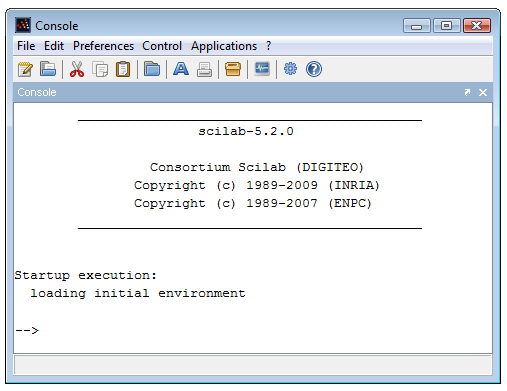
\includegraphics[width=10cm]{introscilab/win32-scilab-console-5-2-0.png}
\end{center}
\caption{Scilab console under Windows.}
\label{fig-win32-scilab-console}
\end{figure}

\subsubsection{Installing Scilab under Linux}

\index{Linux}
Under Linux, the binary versions are available from Scilab 
website as .tar.gz files. There is no need for an installation 
program with Scilab under Linux: simply unzip the file in one target 
directory. Once done, the binary file is located in \emph{<path>/scilab-5.2.0/bin/scilab}.
When this script is executed, the console immediately appears and looks 
exactly the same as on Windows.

Notice that Scilab is also distributed with the packaging system available 
with Linux distributions based on Debian (for example, Ubuntu). 
That installation method is extremely simple and efficient. 
Nevertheless, it has one little drawback: the version of Scilab packaged for your Linux distribution
may not be up-to-date. This is because there is some delay (from 
several weeks to several months) between the availability of an up-to-date version 
of Scilab under Linux and its release in Linux 
distributions.

For now, Scilab comes on Linux with a linear algebra library which is optimized 
and guarantees portability.
Under Linux, Scilab does not come with a binary version of ATLAS \cite{AtlasWWW},
so that linear algebra is a little slower for that platform.

\subsubsection{Installing Scilab under Mac OS}
\index{Mac OS}
Under Mac OS, the binary versions are available from Scilab 
website as a .dmg file. This binary works for Mac OS versions 
starting from version 10.5. It uses the Mac OS installer, which 
provides a classical installation process. 
Scilab is not available on Power PC systems. 

Scilab version 5.2 for Mac OS comes with a Tcl / Tk library which is disabled 
for technical reasons.
As a consequence, there are some small limitations on the 
use of Scilab on this platform. For example, the Scilab / Tcl interface (TclSci), the 
graphic editor and the variable editor are not working.
These features will be rewritten in Java in future versions of 
Scilab and these limitations will disappear.

Still, using Scilab on Mac OS system is easy, and uses the 
shorcuts which are familiar to users of this platform. For example, 
the console and the editor use the Cmd key (Apple key) which is 
found on Mac keyboards. Moreover, there is no right-click 
on this platform. Instead, Scilab is sensitive to the 
Control-Click keyboard event. 

For now, Scilab comes on Mac OS with a linear algebra library which is optimized 
and guarantees portability.
Under Mac OS, Scilab does not come with a binary version of ATLAS \cite{AtlasWWW},
so that linear algebra is a little slower for that platform.

\subsection{How to get help}
\index{\scifun{help}}
The most simple way to get the online help integrated to 
Scilab is to use the function \scifun{help}. 
The figure \ref{fig-scilab-help} presents the Scilab help window.
To use this function, simply type "\scifun{help}" in the console 
and press the <Enter> key, as in the following session.

\lstset{language=scilabscript}
\begin{lstlisting}
help
\end{lstlisting}

\begin{figure}
\begin{center}
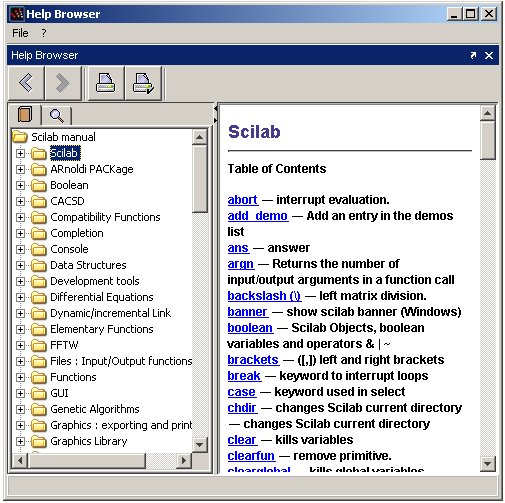
\includegraphics[width=10cm]{introscilab/scilab-help.png}
\end{center}
\caption{Scilab help window.}
\label{fig-scilab-help}
\end{figure}

Suppose that you want some help about the \scifun{optim}
function. You may try to browse the integrated help, find the optimization
section and then click on the \scifun{optim} item
to display its help.

Another possibility is to use the function \scifun{help}, followed 
by the name of the function which help is required, as in the following 
session.
\lstset{language=scilabscript}
\begin{lstlisting}
help optim
\end{lstlisting}
Scilab automatically opens the associated entry
in the help.

We can also use the help provided on Scilab web site
\begin{center}
\url{http://www.scilab.org/product/man}
\end{center}

That page always contains the help for the up-to-date
version of Scilab. By using the "search" feature of my
web browser, I can most of the time quickly find the help 
I need. With that method, I can see the help of several Scilab 
commands at the same time (for example the commands \scifun{derivative}
and \scifun{optim}, so that I can provide the cost function
suitable for optimization with \scifun{optim} by computing
derivatives with \scifun{derivative}).

A list of commercial books, free books, online tutorials and articles 
is presented on the Scilab homepage:
\begin{center}
\url{http://www.scilab.org/publications}
\end{center}

\subsection{Mailing lists, wiki and bug reports}

The mailing list \emph{users@lists.scilab.org} is designed
for all Scilab usage questions. To subscribe to this 
mailing list, send an e-mail to \emph{users-subscribe@lists.scilab.org}.
The mailing list \emph{dev@lists.scilab.org} focuses on the development of Scilab, be 
it the development of Scilab core or of complicated modules which interacts 
deeply with Scilab core.
To subscribe to this mailing list, send an e-mail to \emph{dev-subscribe@lists.scilab.org}.

These mailing lists are archived at:
\begin{center}
\begin{small}
\url{http://dir.gmane.org/gmane.comp.mathematics.scilab.user}
\end{small}
\end{center}
and:
\begin{center}
\begin{small}
\url{http://dir.gmane.org/gmane.comp.mathematics.scilab.devel}
\end{small}
\end{center}

Therefore, before asking a question, users should consider looking in the archive 
if the same question or subject has already been answered.

A question posted on the mailing list may be related to a very specific technical point, so that it requires an
answer which is not general enough to be public. The address 
\emph{scilab.support@scilab.org} is designed for this purpose.
Developers of the Scilab team provide accurate answers via this communication
channel.

The Scilab wiki is a public tool for reading and publishing general information
about Scilab:
\begin{center}
\url{http://wiki.scilab.org}
\end{center}
It is used both by Scilab users and developers to publish 
information about Scilab. From a developer point of view, it contains step-by-step
instructions to compile Scilab from the sources, dependencies of various 
versions of Scilab, instructions to use Scilab source 
code repository, etc...

The Scilab Bugzilla \emph{http://bugzilla.scilab.org} allows to submit 
a report each time we find a new bug. It may happen that this bug has already been
discovered by someone else before. This is why it is advised to search in the bug 
database for existing related problems before reporting a new bug. If the 
bug is not already reported, it is a very good thing to report it, along 
with a test script. This test script should remain as simple as possible, 
which allows to reproduce the problem and identify the source of the issue.

An efficient way of getting up-to-date information is to use RSS feeds.
The RSS feed associated with the Scilab website is 
\begin{center}
\url{http://www.scilab.org/en/rss_en.xml}
\end{center}
This channel delivers regularily press releases and general 
announces.

\subsection{Getting help from Scilab demonstrations and macros}

The Scilab consortium maintains a collection of demonstration scripts,
which are available from the console, in the menu \scimenu{?>Scilab Demonstrations}.
The figure \ref{fig-scilab-demos} presents the demonstration 
window. Some demonstrations are graphic, while some others 
are interactive, which means that the user must type on the 
<Enter> key to go on to the next step of the demo.

\begin{figure}
\begin{center}
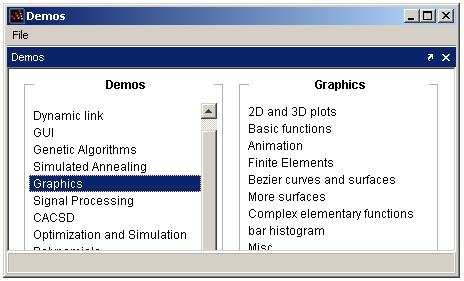
\includegraphics[width=10cm]{introscilab/scilab-demos.png}
\end{center}
\caption{Scilab demos window.}
\label{fig-scilab-demos}
\end{figure}

The associated demonstrations scripts are located in the 
Scilab directory, inside each module. For example, the demonstration
associated with the optimization module is located in the 
file 
\begin{center}
\begin{small}
\begin{verbatim}
<path>\scilab-5.2.0\modules\optimization\demos\datafit\datafit.dem.sce
\end{verbatim}
\end{small}
\end{center}
Of course, the exact path of the file depends on your particular
installation and your operating system.

Analyzing the content of these demonstration files is often 
an efficient solution for solving common problems and to 
understand particular features.

Another method to find some help is to analyze the source code 
of Scilab itself (Scilab is indeed open-source!). 
For example, the \scifun{derivative} function is located in 
\begin{center}
\begin{small}
\begin{verbatim}
<path>\scilab-5.2.0\modules\optimization\macros\derivative.sci
\end{verbatim}
\end{small}
\end{center}

Most of the time, Scilab macros are very well written, taking care 
of all possible combinations of input and output 
arguments and many possible values of the input arguments. 
Often, difficult numerical problems are solved in these scripts so that 
they provide a deep source of inspiration for developing your 
own scripts.


%%%%%%%%%%%%%%%%%%%%%%%%%%%%%%%%%%%%%%%%%%%%%%%%%%%%%%%%%%%%%%%%%
\section{Getting started}

In this section, we make our first steps with Scilab and present 
some simple tasks we can perform with the interpreter.

There are several ways of using Scilab and the following paragraphs
present three methods:
\begin{itemize}
\item using the console in interactive mode,
\item using the \scifun{exec} function against a file,
\item using \emph{batch} processing.
\end{itemize}

\subsection{The console}
\index{console}
The first way is to use Scilab interactively, by typing commands
in the console, analyzing Scilab result, continuing this 
process until the final result is computed. 
This document is designed so that the Scilab examples 
which are printed here can be copied into the console. 
The goal is that the reader can experiment by himself Scilab behavior. 
This is indeed a good way of understanding the behavior of the program and,
most of the time, it allows a quick and smooth way of performing the 
desired computation.

\index{\scifun{disp}}
In the following example, the function \scifun{disp} is 
used in interactive mode to print out the string "Hello World !".
\lstset{language=scilabscript}
\begin{lstlisting}
-->s="Hello World!"
 s  =
 Hello World!   
-->disp(s)
 Hello World!   
\end{lstlisting}

\index{prompt}
In the previous session, we did not type the characters "\verb|-->|" which 
is the \emph{prompt}, and which is managed by Scilab.
We only type the statement \scivar{s="Hello World!"} with our keyboard
and then hit the \scivar{<Enter>} key. Scilab answer is \scivar{ s  =}
and \scivar{Hello World!}. Then we type \scivar{disp(s)} and 
Scilab answer is \scivar{Hello World!}.

When we edit the command, we can use the keyboard, as with a 
regular editor. We can use the left $\leftarrow$ and right $\rightarrow$ arrows
in order to move the cursor on the line and use the <Backspace> and <Suppr> keys
in order to fix errors in the text.

In order to get an access to previously executed commands, 
use the up arrow $\uparrow$ key. This allows to browse the previous 
commands by using the up $\uparrow$ and down $\downarrow$ arrow keys. 

The <Tab> key provides a very convenient completion feature. 
In the following session, we type the statement \scifun{disp} in the console.
\lstset{language=scilabscript}
\begin{lstlisting}
-->disp
\end{lstlisting}

Then we can type on the <Tab> key, which makes a list appear in the 
console, as presented in the figure \ref{fig-scilab-console}.
Scilab displays a listbox, where items correspond to all functions
which begin with the letters "disp". 
We can then use the up and down arrow keys to select the function 
we want.

\begin{figure}
\begin{center}
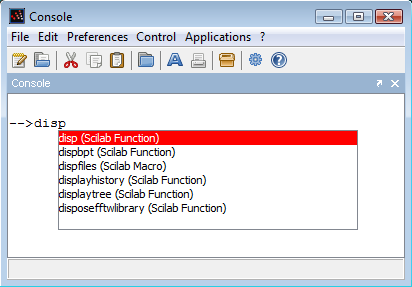
\includegraphics[width=10cm]{introscilab/console_completion.png}
\end{center}
\caption{The completion in the console.}
\label{fig-scilab-console}
\end{figure}

The auto-completion works with functions, variables, files and graphic 
handles and makes the development of scripts easier and faster.

\subsection{The editor}

Scilab version 5.2 provides a new editor which allows to edit scripts easily. 
The figure \ref{fig-scilab-editorhelloworld} presents the editor while 
it is editing the previous "Hello World!" example.

\begin{figure}
\begin{center}
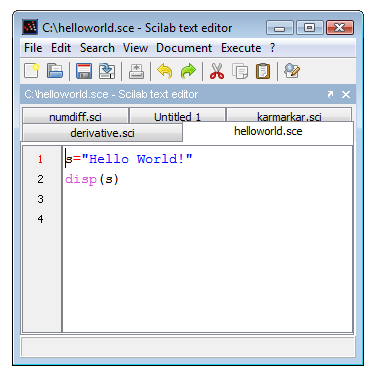
\includegraphics[width=10cm]{introscilab/editor-helloworld.png}
\end{center}
\caption{The editor.}
\label{fig-scilab-editorhelloworld}
\end{figure}

The editor can be accessed from the menu of the console, under 
the \scimenu{Applications > Editor} menu, or from the console, 
as presented in the following session.
\lstset{language=scilabscript}
\begin{lstlisting}
-->editor()
\end{lstlisting}

This editor allows to manage several files at the same time, as 
presented in the figure \ref{fig-scilab-editorhelloworld}, where 
we edit five files at the same time. 

There are many features which are worth to mention in this editor. 
The most commonly used features are under the \scimenu{Execute} menu.
\begin{itemize}
\item \scimenu{Load into Scilab} allows to execute the statements in the 
current file, as if we did a copy and paste. This implies that the 
statements which do not end with a ";" character will produce an output 
in the console.
\item \scimenu{Evaluate Selection} allows to execute the statements which 
are currently selected.
\item \scimenu{Execute File Into Scilab} allows to execute the file, as 
if we used the \scifun{exec} function. The results which are produced 
in the console are only those which are associated with printing 
functions, such as \scifun{disp} for example.
\end{itemize}
We can also select a few lines in the script, right click (or Cmd+Click
under Mac), and get the context menu which is presented in figure \ref{fig-scilab-contextmenu}.

\begin{figure}
\begin{center}
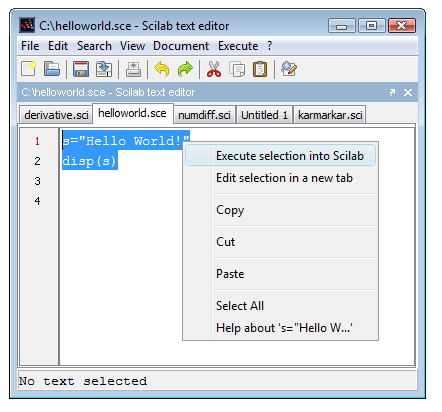
\includegraphics[width=10cm]{introscilab/editor-rightclick.png}
\end{center}
\caption{Context menu in the editor.}
\label{fig-scilab-contextmenu}
\end{figure}

The \scimenu{Edit} menu provides a very interesting feature, commonly
known as a "pretty printer" in most languages. This is the 
\scimenu{Edit > Correct Indentation} feature, which automatically
indents the current selection. This feature is extremelly convenient,
as it allows to format algorithms so that the \scifun{if}, 
\scifun{for} and other structured blocks can be 
easy to analyze.

The editor provides a fast access to the inline help. 
Indeed, assume that we have selected the \scifun{disp} statement, 
as presented in the figure \ref{fig-scilab-contexthelp}. 
When we right-click in the editor, we get the context menu,
where the \scimenu{Help about "disp"} entry allows to open the help associated with the \scifun{disp} 
function.

\begin{figure}
\begin{center}
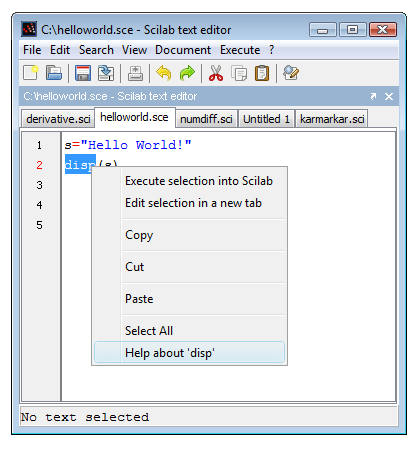
\includegraphics[width=7cm]{introscilab/editor-help.png}
\end{center}
\caption{Context help in the editor.}
\label{fig-scilab-contexthelp}
\end{figure}

\subsection{Docking}
\index{docking}
The graphics in Scilab version 5 has been updated so that many 
components are now based on Java. This has a number of advantages,
including the possibility to manage docking windows.

The docking system uses Flexdock \cite{FlexdockWWW}, an open-source project 
providing a Swing docking framework. Assume that we have both the 
console and the editor opened in our environment, as presented in figure 
\ref{fig-scilab-consoledock}. It might be annoying to manage two 
windows, because one may hide the other, so that we constantly have 
to move them around in order to actually see what happens. 

\index{Flexdock}
The Flexdock system allows to drag and drop the editor into the console, so that we finally have only one 
window, with several sub-windows. All Scilab windows are dockable, including
the console, the editor, the help and the plotting windows. In the figure 
\ref{fig-scilab-consoleundock}, we present a situation where we have docked 
four windows into the console window.

\begin{figure}
\begin{center}
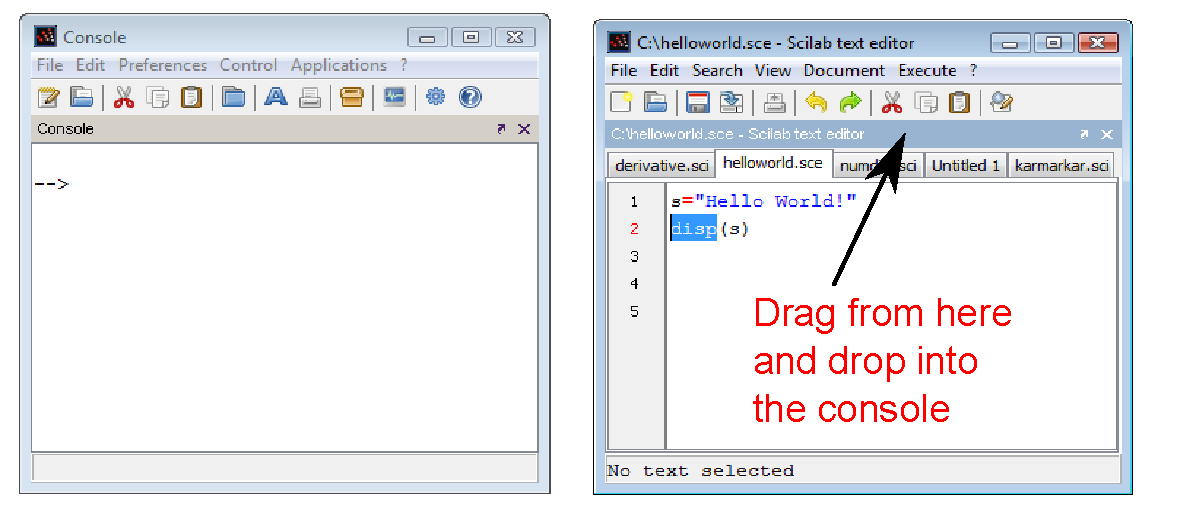
\includegraphics[width=10cm]{introscilab/console-dock.pdf}
\end{center}
\caption{The title bar in the source window. In order to dock the editor into the 
console, drag and drop the title bar of the editor into the console.}
\label{fig-scilab-consoledock}
\end{figure}

\begin{figure}
\begin{center}
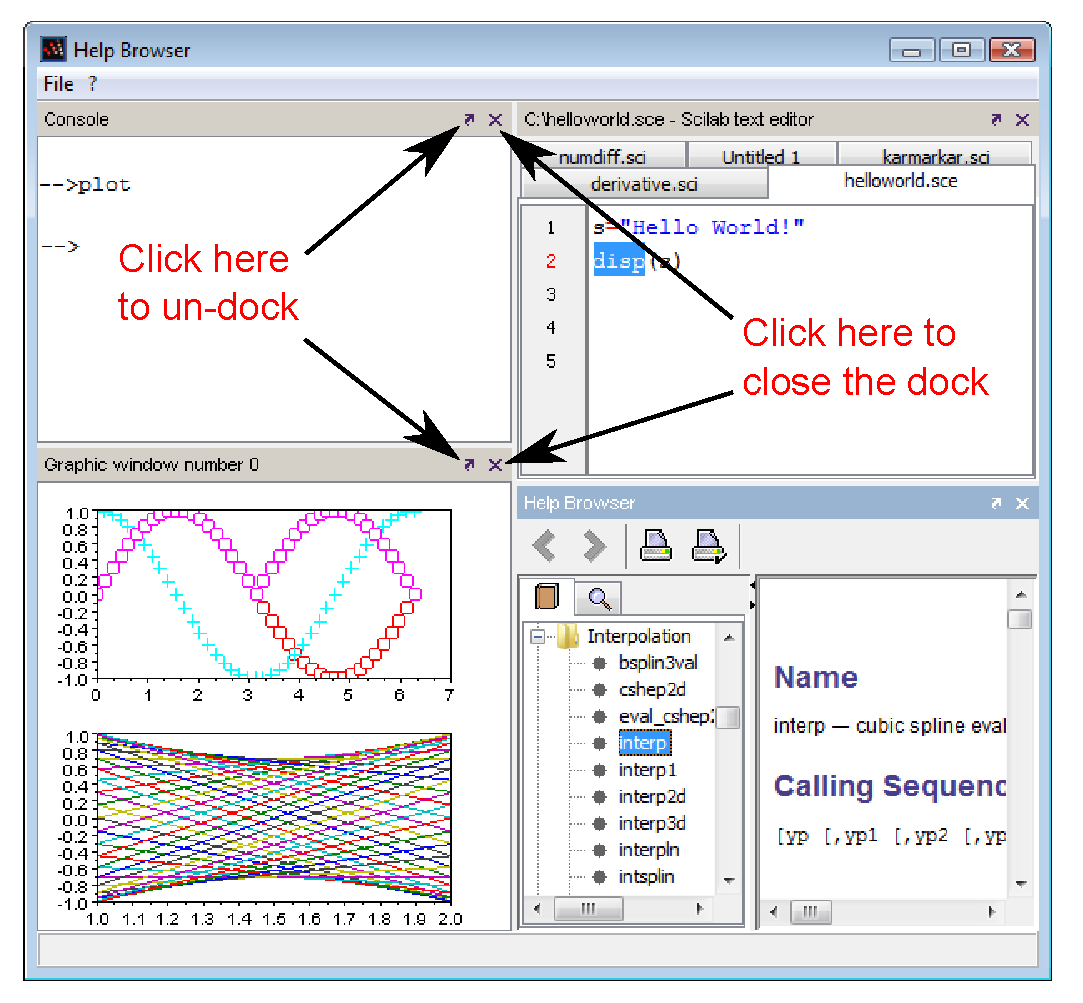
\includegraphics[width=10cm]{introscilab/console-undock.pdf}
\end{center}
\caption{Actions in the title bar of the docking window. The round arrow in the 
title bar of the window allows to undock the window. The cross allows to 
close the window.}
\label{fig-scilab-consoleundock}
\end{figure}

In order to dock one window into another window, we must drag and 
drop the source window into the target window. To do this, we 
left-click on the title bar of the docking window, as indicated 
in figure \ref{fig-scilab-consoledock}. Before releasing the 
click, let us move the mouse over the target window and notice that 
a window, surrounded by dotted lines is displayed. This "fantom" 
window indicates the location of the future docked window. We can 
choose this location, which can be on the top, the bottom, the left
or the right of the target window. Once we have chosen the target location,
we release the click, which finally moves the source window into the 
target window, as in the figure \ref{fig-scilab-consoleundock}.

We can also release the source window \emph{over} the target window,
which creates tabs, as in the figure \ref{fig-scilab-docktabs}.

\begin{figure}
\begin{center}
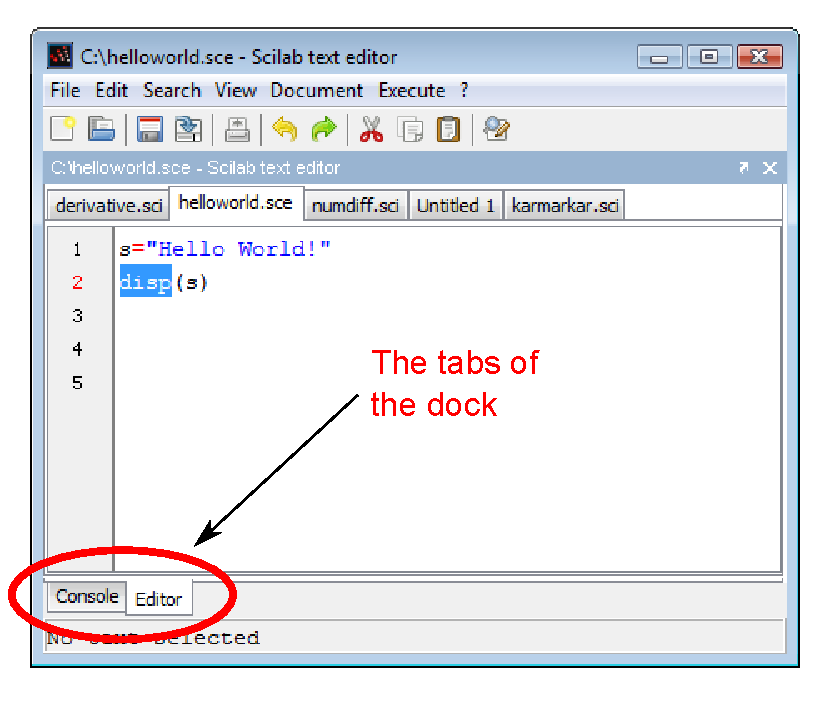
\includegraphics[width=10cm]{introscilab/console-docktabs.pdf}
\end{center}
\caption{Docking tabs.}
\label{fig-scilab-docktabs}
\end{figure}

\subsection{Using \scifun{exec}}
When several commands are to be executed, it may be 
more convenient to write these statements into a file with
Scilab editor.
To execute the commands located in such a file, the \scifun{exec}
function can be used, followed by the name of the script.
This file generally has the extension .sce or .sci, depending
on its content: 
\begin{itemize}
\item files having the .sci extension are containing Scilab functions and 
executing them loads the functions into Scilab environment (but does not 
execute them),
\item files having the .sce extension are containing both Scilab functions and 
executable statements.
\end{itemize}
Executing a .sce file has generally an effect such 
as computing several variables and displaying the results in the console, 
creating 2D plots, reading or writing into a file, etc...

Assume that the content of the file \emph{myscript.sce} is 
the following.
\lstset{language=scilabscript}
\begin{verbatim}
disp("Hello World !")
\end{verbatim}

In the Scilab console, we can use the \emph{exec} function 
to execute the content of this script.
\lstset{language=scilabscript}
\begin{lstlisting}
-->exec("myscript.sce")
-->disp("Hello World !")
 Hello World !   
\end{lstlisting}

In practical situations such as debugging a complicated algorithm, 
the interactive mode is most of the time used with a sequence 
of calls to the \scifun{exec} and \scifun{disp} functions.

\subsection{Batch processing}
Another way of using Scilab is from the command line. 
Several command line options are available and are presented in 
figure \ref{fig-scilab-commandlineoptions}. 
Whatever the operating system is, binaries are located in the directory 
\emph{scilab-5.2.0/bin}.
Command line options must be appended to the binary for 
the specific platform, as described below.
The \emph{-nw} option allows to disable the display of the console. 
The \emph{-nwni} option allows to launch the non-graphics mode: in this mode, the console 
is not displayed and plotting functions are disabled (using them will generate an 
error).

\begin{itemize}
\item Under Windows, two binary executable are provided. The first executable is \emph{WScilex.exe}, 
the usual, graphics, interactive console. This executable corresponds to 
the icon which is available on the desktop after the installation of Scilab.
The second executable is \emph{Scilex.exe}, the non-graphics console. With the 
\emph{Scilex.exe} executable, the Java-based console is not loaded and the Windows terminal 
is directly used. The \emph{Scilex.exe} program is sensitive to the \emph{-nw}
and \emph{-nwni} options.

\item Under Linux, the \emph{scilab} script provides options which 
allow to configure its behavior. By default, the graphics mode is 
launched. The \emph{scilab} script is sensitive to the \emph{-nw}
and \emph{-nwni} options.
There are two extra executables on Linux: \emph{scilab-cli} and \emph{scilab-adv-cli}.
The \emph{scilab-adv-cli} executable is equivalent to the \emph{-nw} option,
while the \emph{scilab-cli} is equivalent to the \emph{-nwni} option\cite{WikiNwniWWW}.

\item Under Mac OS, the behavior is similar to the Linux platform.
\end{itemize}

In the following Windows session, we launch the \emph{Scilex.exe}
program with the \emph{-nwni} option. Then we run the \scifun{plot}
function in order to check that this function is not available 
in the non-graphics mode.
\begin{lstlisting}
D:\Programs\scilab-5.2.0\bin>Scilex.exe -nwni
        ___________________________________________
                       scilab-5.2.0
                 Consortium Scilab (DIGITEO)
               Copyright (c) 1989-2009 (INRIA)
               Copyright (c) 1989-2007 (ENPC)
        ___________________________________________
Startup execution:
  loading initial environment
-->plot()
       !--error 4
Undefined variable: plot
\end{lstlisting}

\index{\scivar{SCIHOME}}
\begin{figure}
\begin{center}
\begin{tabular}{|l|l|}
\hline
-e instruction & execute the Scilab instruction given in instruction\\
\hline
-f file & execute the Scilab script given in the file\\
\hline
-l lang &  setup the user language \\
&'fr' for french and 'en' for english (default is 'en')\\
\hline
-mem N & set the initial stacksize.\\
\hline
-ns & if this option is present, the startup file scilab.start is not executed.\\
\hline
-nb & if this option is present, then Scilab welcome banner is not displayed.\\
\hline
-nouserstartup & don't execute user startup files SCIHOME/.scilab \\
& or SCIHOME/scilab.ini.\\
\hline
-nw & start Scilab as command line with advanced features (e.g., graphics).\\
\hline
-nwni & start Scilab as command line without advanced features.\\
\hline
-version & print product version and exit.\\
\hline
\end{tabular}
\end{center}
\caption{Scilab command line options.}
\label{fig-scilab-commandlineoptions}
\end{figure}

\index{batch}
The most useful command line option is the -f option, which 
allows to execute the commands from a given file, a method 
generally called \emph{batch} processing. 
Assume that the content of the file \emph{myscript2.sce} is 
the following, where the \scifun{quit} function is used 
to exit from Scilab.
\lstset{language=scilabscript}
\begin{lstlisting}
disp("Hello World !")
quit()
\end{lstlisting}

The default behavior of Scilab is to wait for new user input: 
this is why the \scifun{quit} command is used, so that the 
session terminates.
To execute the demonstration under Windows, we created the directory "C:\textbackslash scripts"
and wrote the statements in the file 
\emph{C:\textbackslash scripts\textbackslash myscript2.sce}.
The following session, executed from the MS Windows terminal, 
shows how to use the -f option to execute the previous script.
Notice that we used the absolute path of the \emph{Scilex.exe} executable.
\begin{lstlisting}
C:\scripts>D:\Programs\scilab-5.2.0\bin\Scilex.exe -f myscript2.sce
        ___________________________________________
                       scilab-5.2.0
                 Consortium Scilab (DIGITEO)
               Copyright (c) 1989-2009 (INRIA)
               Copyright (c) 1989-2007 (ENPC)
        ___________________________________________
Startup execution:
  loading initial environment
 Hello World !
C:\scripts>
\end{lstlisting}

\index{comment}
Any line which begins with the two characters "//" is considered
by Scilab as a comment and is ignored.
To check that Scilab stays by default in interactive mode, we comment out 
the \scifun{quit} statement with the "//" syntax, as in the following 
script.
\lstset{language=scilabscript}
\begin{lstlisting}
disp("Hello World !")
//quit()
\end{lstlisting}

If we type the "scilex -f myscript2.sce" command in the terminal, 
Scilab waits now for user input, as expected. To exit, we 
interactively type the \scifun{quit()} statement in the 
terminal.


%%%%%%%%%%%%%%%%%%%%%%%%%%%%%%%%%%%%%%%%%%%%%%%%%%%%%%%%%%%%%%%%%
\section{Basic elements of the language}

Scilab is an interpreted language, which means  
that it allows to manipulate variables in a very 
dynamic way. In this section, we present the basic 
features of the language, that is, we show how to create a real variable,
and what elementary mathematical functions 
can be applied to a real variable. If Scilab provided only these
features, it would only be a super desktop calculator. 
Fortunately, it is a lot more and this is the subject of the remaining
sections, where we will show how to manage other 
types of variables, that is booleans, complex numbers, integers
and strings.

It seems strange at first, but it is worth to state it
right from the start: \emph{in Scilab, everything is a matrix}.
To be more accurate, we should write: \emph{all real, complex,
boolean, integer, string and polynomial variables are matrices}. 
Lists and other complex data structures (such as tlists and mlists) 
are not matrices (but can contain matrices). These complex data 
structures will not be presented in this document.

This is why we could begin by presenting matrices.
Still, we choose to present basic data types first, because 
Scilab matrices are in fact a special organization of these 
basic building blocks.

In Scilab, we can manage real and complex numbers. This always 
leads to some confusion if the context is not clear enough.
In the following, when we write \emph{real variable}, we will 
refer to a variable which content is not complex. Complex variables
will be covered in section \ref{introscilab-complexnumber} as 
a special case of real variables. In most cases, 
real variables and complex variables behave in a very similar way,
although some extra care must be taken when complex data is to 
be processed. Because it would make the presentation cumbersome, 
we simplify most of the discussions by considering only real variables,
taking extra care with complex variables only when needed.

%%%%%%%%%%%%%%%%%%%%%%%%%%%%%%%%%%%%%%%%%%%%%%%%%%%%%%%%%%%%%%%%%%%%%%%
\subsection{Creating real variables}

In this section, we create real variables and perform simple operations with 
them.
 
Scilab is an interpreted language, which implies that 
there is no need to declare a variable before using it.
Variables are created at the moment where they are first set. 

In the following example, we create and set the real variable $x$ to 1
and perform a multiplication on this variable.
In Scilab, the "=" operator means that we want to set the variable on the 
left hand side to the value associated to the right hand side (it is 
not the comparison operator, which syntax is associated to the "==" operator).
\lstset{language=scilabscript}
\begin{lstlisting}
-->x=1
 x  =
    1.  
-->x = x * 2
 x  =
    2.  
\end{lstlisting}

\index{semicolon}
\index{\scifun{;}}
The value of the variable is displayed each time a statement is executed.
That behavior can be suppressed if the line ends  
with the semicolon ";" character, as in the following example.

\lstset{language=scilabscript}
\begin{lstlisting}
-->y=1;
-->y=y*2;
\end{lstlisting}

\index{hat}
\index{$\hat{\;}$}
All the common algebraic operators presented in figure \ref{fig-introscilab-elemenop}
are available in Scilab. Notice that the power operator is represented 
by the hat "$\hat{\;}$" character so that computing $x^2$ in Scilab is performed 
by the "x$\hat{\;}$2" expression or equivalently by the "x**2" expression.
The single quote operator \scisinglequote{} will be presented in more depth in section \ref{introscilab-complexnumber}, which 
presents complex numbers.

\begin{figure}
\begin{center}
\begin{tabular}{|ll|}
\hline
+ & addition \\
- & substraction \\
\textasteriskcentered & multiplication \\
/ & right division i.e. $x/y=xy^{-1}$\\
$\backslash$ & left division i.e. $x\backslash y=x^{-1}y$\\
$\hat{\;}$ & power i.e. $x^y$\\
\textasteriskcentered\textasteriskcentered & power (same as $\hat{\;}$)\\
' & transpose conjugate \\
\hline
\end{tabular}
\end{center}
\caption{Scilab mathematical elementary operators.}
\label{fig-introscilab-elemenop}
\end{figure}

%%%%%%%%%%%%%%%%%%%%%%%%%%%%%%%%%%%%%%%%%%%%%%%%%%%%%%%%%%%%%%%%%%%%%%%
\subsection{Variable name}

\index{variable name}
Variable names may be as long as the user wants, but only the first 24 characters 
are taken into account in Scilab. For consistency, we should consider
only variable names which are not made of more than 24 characters.
All ASCII letters from "a" to "z", from "A" to "Z" and from "0" to "9" 
are allowed, with the additional letters "\%", "\_", "\#", "!", "\$", "?".
Notice though that variable names which first letter is "\%" have 
a special meaning in Scilab, as we will see in section \ref{introscilab-predefinedvars},
which presents the mathematical pre-defined variables.

Scilab is case sensitive, which means that upper and lower case letters are 
considered to be different by Scilab.
In the following script, we define the two variables \scivar{A}
and \scivar{a} and check that these two variables are considered 
to be different by Scilab.
\lstset{language=scilabscript}
\begin{lstlisting}
-->A = 2
 A  =
    2.  
-->a = 1
 a  =
    1.  
-->A
 A  =
    2.  
-->a
 a  =
    1.  
\end{lstlisting}

%%%%%%%%%%%%%%%%%%%%%%%%%%%%%%%%%%%%%%%%%%%%%%%%%%%%%%%%%%%%%%%%%%%%%%%
\subsection{Comments and continuation lines}

\index{comment}
\index{\scifun{//}}
Any line which begins with two slashes "//" is considered 
by Scilab as a comment and is ignored. There is no possibility 
to comment out a block of lines, such as with the "/* ... */" comments
in the C language.

\index{continuation line}
\index{dot}
\index{\scifun{..}}
When an executable statement is too long to be written on a single line,
the second line and above are called continuation lines.
In Scilab, any line which ends with two dots is considered
to be the start of a new continuation line. 
In the following session, we give examples of Scilab comments
and continuation lines.
\lstset{language=scilabscript}
\begin{lstlisting}
-->// This is my comment.
-->x=1..
-->+2..
-->+3..
-->+4
 x  =
    10.  
\end{lstlisting}

%%%%%%%%%%%%%%%%%%%%%%%%%%%%%%%%%%%%%%%%%%%%%%%%%%%%%%%%%%%%%%%%%%%%%%%
\subsection{Elementary mathematical functions}

\index{elementary functions}
The tables \ref{fig-introscilab-elemenfun1} and \ref{fig-introscilab-elemenfun2} 
present a list of elementary mathematical functions.
Most of these functions take one input argument and return one output argument.
These functions are vectorized in the sense that their input and output arguments 
are matrices. This allows to compute data with higher performance, without 
any loop.

In the following example, we use the \scifun{cos} and \scifun{sin} functions and 
check the equality $\cos(x)^2+\sin(x)^2=1$.
\lstset{language=scilabscript}
\begin{lstlisting}
-->x = cos(2)
 x  =
  - 0.4161468  
-->y = sin(2)
 y  =
    0.9092974  
-->x^2+y^2
 ans  =
    1.  
\end{lstlisting}


\begin{figure}
\begin{center}
\begin{tabular}{|llllllll|}
\hline
    acos   &    acosd   &    acosh  &    acoshm  &    acosm  &    acot   &    acotd   &    acoth  \\
    acsc   &    acscd   &    acsch  &    asec    &    asecd  &    asech  &    asin    &    asind  \\
    asinh  &    asinhm  &    asinm  &    atan    &    atand  &    atanh  &    atanhm  &    atanm  \\
    cos    &    cosd    &    cosh   &    coshm   &    cosm   &    cotd   &    cotg    &    coth   \\
    cothm  &    csc     &    cscd   &    csch    &    sec    &    secd   &    sech    &    sin    \\
    sinc    &    sind   &    sinh   &    sinhm   &    sinm   &    tan    &    tand    &    tanh  \\
    tanhm  &    tanm  &&&&&&\\
\hline
\end{tabular}
\end{center}
\caption{Scilab mathematical elementary functions: trigonometry.}
\label{fig-introscilab-elemenfun1}
\end{figure}


\begin{figure}
\begin{center}
\begin{tabular}{|llllllll|}
\hline
    exp   &    expm  &    log   &    log10   &    log1p   &    log2  &    logm  &    max  \\
    maxi  &    min   &    mini  &    modulo  &    pmodulo &    sign  &    signm &    sqrt  \\
    sqrtm  & &&&&&&\\
\hline
\end{tabular}
\end{center}
\caption{Scilab mathematical elementary functions: other functions.}
\label{fig-introscilab-elemenfun2}
\end{figure}

%%%%%%%%%%%%%%%%%%%%%%%%%%%%%%%%%%%%%%%%%%%%%%%%%%%%%%%%%%%%%%%%%%%%%%%
\subsection{Pre-defined mathematical variables}
\label{introscilab-predefinedvars}

In Scilab, several mathematical variables are pre-defined variables, 
which name begins with a percent "\%" character.
The variables which have a mathematical meaning are 
summarized in figure \ref{fig-introscilab-glovarmath}.

\begin{figure}
\begin{center}
\begin{tabular}{|ll|}
\hline
\%i & the imaginary number $i$\\
\%e & Euler's constant $e$\\ 
\%pi & the mathematical constant $\pi$\\
\hline
\end{tabular}
\end{center}
\caption{Pre-defined mathematical variables.}
\label{fig-introscilab-glovarmath}
\end{figure}

\index{\scivar{\%pi}}
In the following example, we use the variable
\scivar{\%pi} to check the mathematical equality $\cos(x)^2 + \sin(x)^2 = 1$.
\lstset{language=scilabscript}
\begin{lstlisting}
-->c=cos(%pi)
 c  =
  - 1.  
-->s=sin(%pi)
 s  =
    1.225D-16  
-->c^2+s^2
 ans  =
    1.  
\end{lstlisting}

The fact that the computed value of $\sin(\pi)$ is \emph{not exactly} 
equal to 0 is a consequence of the fact that 
Scilab stores the real numbers with floating point numbers,
that is, with limited precision. 

%%%%%%%%%%%%%%%%%%%%%%%%%%%%%%%%%%%%%%%%%%%%%%%%%%%%%%%%%%%%%%%%%%%%%%%
\subsection{Booleans}

\index{boolean}
Boolean variables can store true or false values. In Scilab, true is written with 
"\%t" or "\%T" and false is written with "\%f" or "\%F".
The figure \ref{fig-introscilab-compoperators} presents the 
several comparison operators which are available in Scilab.
These operators return boolean values and take as input arguments 
all basic data types (i.e. real and complex numbers, integers and strings).

\begin{figure}
\begin{center}
\begin{tabular}{|ll|}
\hline
a\&b & logical and\\
a|b & logical or\\
$\thicksim$a & logical not\\
a==b & true if the two expressions are equal\\
a$\thicksim$=b or a<>b& true if the two expressions are different\\
a<b & true if a is lower than b\\
a>b & true if a is greater than b\\
a<=b & true if a is lower or equal to b\\
a>=b & true if a is greater or equal to b\\
\hline
\end{tabular}
\end{center}
\caption{Comparison operators.}
\label{fig-introscilab-compoperators}
\end{figure}

In the following example, we perform some algebraic computations 
with Scilab booleans.

\lstset{language=scilabscript}
\begin{lstlisting}
-->a=%T
 b  =
  T  
-->b = ( 0 == 1 )
 a  =
  F  
-->a&b
 ans  =
  F  
\end{lstlisting}

%%%%%%%%%%%%%%%%%%%%%%%%%%%%%%%%%%%%%%%%%%%%%%%%%%%%%%%%%%%%%%%%%%%%%%%
\subsection{Complex numbers}
\label{introscilab-complexnumber}

\index{complex number}
\index{\scivar{\%i}}
Scilab provides complex numbers, which are stored 
as pairs of floating point numbers. 
The pre-defined variable \scivar{\%i} represents the mathematical imaginary
number $i$ which satisfies $i^2=-1$.
All elementary functions previously presented before, such as \scifun{sin} for example, 
are overloaded for complex numbers. This means that, if their input 
argument is a complex number, the output is a complex 
number. The figure \ref{fig-introscilab-complexelemfun} presents  
functions which allow to manage complex numbers.

\begin{figure}
\begin{center}
\begin{tabular}{|ll|}
\hline
real & real part \\
imag & imaginary part \\
imult & multiplication by $i$, the imaginary unitary \\
isreal & returns true if the variable has no complex entry \\
\hline
\end{tabular}
\end{center}
\caption{Scilab complex numbers elementary functions.}
\label{fig-introscilab-complexelemfun}
\end{figure}

In the following example, we set the variable $x$ to $1+i$,
and perform several basic operations on it, such as retrieving 
its real and imaginary parts. Notice how the single quote operator, 
denoted by \scisinglequote{},  is used to compute the conjugate of a complex number.
\lstset{language=scilabscript}
\begin{lstlisting}
-->x= 1+%i
 x  =
    1. + i    
-->isreal(x)
 ans  =
  F  
-->x'
 ans  =
    1. - i    
-->y=1-%i
 y  =
    1. - i    
-->real(y)
 ans  =
    1.  
-->imag(y)
 ans  =
  - 1.  
\end{lstlisting}

We finally check that the equality $(1+i)(1-i)=1-i^2=2$
is verified by Scilab.
\lstset{language=scilabscript}
\begin{lstlisting}
-->x*y
 ans  =
    2.  
\end{lstlisting}


%%%%%%%%%%%%%%%%%%%%%%%%%%%%%%%%%%%%%%%%%%%%%%%%%%%%%%%%%%%%%%%

\subsection{Strings}

\index{string}
Strings can be stored in variables, provided that they are 
delimited by double quotes \scidoublequote{}. 
The concatenation operation is available from the "+" operator. 
In the following Scilab session, we define two strings and then
concatenate them with the "+" operator.
\lstset{language=scilabscript}
\begin{lstlisting}
-->x = "foo"
 x  =
 foo   
-->y="bar"
 y  =
 bar   
-->x+y
 ans  =
 foobar   
\end{lstlisting}

They are many functions which allow to process strings, including 
regular expressions. We will not give further details about this 
topic in this document.

\subsection{Dynamic type of variables}

When we create and manage variables, Scilab allows to change 
the type of a variable dynamically. This means that we can create 
a real value, and then put a string variable in it, as presented 
in the following session.
\lstset{language=scilabscript}
\begin{lstlisting}
-->x=1
 x  =
    1.  
-->x+1
 ans  =
    2.  
-->x="foo"
 x  =
 foo   
-->x+"bar"
 ans  =
 foobar   
\end{lstlisting}

We emphasize here that Scilab is not a typed language, that is, we do not have to declare 
the type of a variable before setting its content. 
Moreover, the type of a variable can change during the life 
of the variable.

%%%%%%%%%%%%%%%%%%%%%%%%%%%%%%%%%%%%%%%%%%%%%%%%%%%%%%%%%%%%%%%%%
\section{Matrices}

\index{matrix}
In the Scilab language, matrices play 
a central role. In this section, we introduce Scilab 
matrices and present how to create and query matrices. We also analyze 
how to access to elements of a matrix, either element by element,
or by higher level operations.

\subsection{Overview}

In Scilab, the basic data type is the matrix, which is defined by:
\begin{itemize}
\item the number of rows,
\item the number of columns,
\item the type of data.
\end{itemize}
The data type can be real, integer, boolean, string and polynomial.
\index{shape}
When two matrices have the same number of rows and columns,
we say that the two matrices have the same \emph{shape}.

In Scilab, vectors are a particular case of matrices,
where the number of rows (or the number of columns) is equal to 1.
Simple scalar variables do not exist in Scilab:
a scalar variable is a matrix with 1 row and 1 column.
This is why in this chapter, when we analyze the behavior of Scilab 
matrices, there is the same behavior for row or column vectors 
(i.e. $n\times 1$ or $1\times n$ matrices) as well as scalars 
(i.e. $1\times 1$ matrices).

It is fair to say that Scilab was designed mainly for matrices of 
\emph{real} variables. This allows to perform linear algebra operations with 
a high level language. 

By design, Scilab was created to be able to perform
matrices operations as fast as possible. The building block for this feature 
is that Scilab matrices are stored in an internal data structure 
which can be managed at the interpreter level.
Most basic linear algebra operations, such as addition, substraction,
transpose or dot product are performed by a compiled, optimized, source code.
These operations are performed with the common operators "\scivar{+}", "\scivar{-}", "\scivar{*}" and the single 
quote \scisinglequote{}, so that, at the Scilab level, the source code is both simple and fast.

With these high level operators, most matrix algorithms do not require to 
use loops. In fact, a Scilab script which performs the same operations
with loops is typically from 10 to 100 times slower.
This feature of Scilab is known as the \emph{vectorization}.
%% which is developped in section \ref{introscilab-section-performances}.
In order to get a fast implementation of a given algorithm, the Scilab 
developper should always use high level operations, so that each statement
process a matrix (or a vector) instead of a scalar.

More complex tasks of linear algebra, such as the resolution of systems of 
linear equations $Ax=b$, various decompositions (for example Gauss 
partial pivotal $PA=LU$), eigenvalue/eigenvector computations, are also
performed by compiled and optimized source codes. These operations 
are performed by common operators like the slash "/" or backslash "$\backslash$" 
or with functions like \scifun{spec},
which computes eigenvalues and eigenvectors.

%%%%%%%%%%%%%%%%%%%%%%%%%%%%%%%%%%%%%%%%%%%%%%%%%%%%%%%%%%%%%%%%%
\subsection{Create a matrix of real values}

There is a simple and efficient syntax to create a matrix with given values.
The following is the list of symbols used to define a matrix:
\begin{itemize}
\item square brackets "[" and "]" mark the beginning and the end of the matrix, 
\item commas "," separate the values on different columns,
\item semicolons ";" separate the values of different rows. 
\end{itemize}
The following syntax can be used to define a matrix, where 
blank spaces are optional (but make the line easier to read) and 
"..." are designing intermediate values:
\lstset{language=scilabscript}
\begin{lstlisting}
A = [a11, a12, ..., a1n; a21, a22, ..., a2n; ...; an1, an2, ..., ann].
\end{lstlisting}
In the following example, we create a $2\times 3$ matrix of real values.
\lstset{language=scilabscript}
\begin{lstlisting}
-->A = [1 , 2 , 3 ; 4 , 5 , 6]
 A  =
    1.    2.    3.  
    4.    5.    6.  
\end{lstlisting}
A simpler syntax is available, which does not require to use the comma
and semicolon characters.
When creating a matrix, the blank space separates the 
columns while the new line separates the 
rows, as in the following syntax:
\lstset{language=scilabscript}
\begin{lstlisting}
A = [a11 a12 ... a1n
a21 a22 ... a2n
...
an1 an2 ... ann]
\end{lstlisting}
This allows to lighten considerably the management of matrices,
as in the following session.
\lstset{language=scilabscript}
\begin{lstlisting}
-->A = [1 2 3
-->4 5 6]
 A  =
    1.    2.    3.  
    4.    5.    6.  
\end{lstlisting}

The previous syntax for matrices is useful in the situations
where matrices are to be written into data files, because it 
simplifies the human reading (and checking) of the values in the file,
and simplifies the reading of the matrix in Scilab.


\begin{figure}
\begin{center}
\begin{tabular}{|ll|}
\hline
eye & identity matrix \\
linspace & linearly spaced vector \\
ones & matrix made of ones \\
zeros & matrix made of zeros \\
testmatrix & generate some particular matrices \\
grand & random number generator \\
rand & random number generator \\
\hline
\end{tabular}
\end{center}
\caption{Functions which generate matrices.}
\label{fig-introscilab-genmatrix}
\end{figure}

Several Scilab commands allow to create matrices from a given 
size, i.e. from a given number of rows and columns. These functions 
are presented in figure \ref{fig-introscilab-genmatrix}.
The most commonly used are \scifun{eye}, \scifun{zeros} and \scifun{ones}.
These commands takes two input arguments, the number of rows and columns of the 
matrix to generate.
\lstset{language=scilabscript}
\begin{lstlisting}
-->A = ones(2,3)
 A  =
    1.    1.    1.  
    1.    1.    1.  
\end{lstlisting}

%%%%%%%%%%%%%%%%%%%%%%%%%%%%%%%%%%%%%%%%%%%%%%%%%%%%%%%%%%%%%%%%%%%%%%%%%%%%%%%%%%%%%%%%%%%%%%%%%%%%
\subsection{The empty matrix \scivar{[]}}

An empty matrix can be created by using empty square brackets, as  
in the following session, where we create a $0\times 0$ matrix.
\lstset{language=scilabscript}
\begin{lstlisting}
-->A=[]
 A  =
     []
\end{lstlisting}

This syntax allows to delete the content of a matrix, so that the 
associated memory is deleted. 
\lstset{language=scilabscript}
\begin{lstlisting}
-->A = ones(100,100);
-->A = []
 A  =
     []
\end{lstlisting}


%%%%%%%%%%%%%%%%%%%%%%%%%%%%%%%%%%%%%%%%%%%%%%%%%%%%%%%%%%%%%%%%%%%%%%%%%%%%%%%%%%%%%%%%%%%%%%%%%%%%
\subsection{Query matrices}

The functions in figure \ref{fig-introscilab-querymatrix} allow 
to query or update a matrix.

\index{\scifun{size}}
The \scifun{size} function returns the two output arguments \scivar{nr}
and \scivar{nc}, which are the number of rows and the number of columns.

\lstset{language=scilabscript}
\begin{lstlisting}
-->A = ones(2,3)
 A  =
    1.    1.    1.  
    1.    1.    1.  
-->[nr,nc]=size(A)
 nc  =
    3.  
 nr  =
    2.  
\end{lstlisting}

The \scifun{size} function is of important practical value when we 
design a function, since the processing 
that we must perform on a given matrix may depend on its shape.
For example, to compute the norm of a given matrix, different algorithms 
may be use depending if the matrix is either a column vector with size $nr\times 1$
and $nr>0$, a row vector with size $1\times nc$ and $nc>0$, or a general matrix 
with size $nr\times nc$ and $nr,nc>0$.

The \scifun{size} function has also the following syntax
\lstset{language=scilabscript}
\begin{lstlisting}
nr = size( A , sel )
\end{lstlisting}
which allows to get only the number of rows or the number of columns and 
where \scivar{sel} can have the following values
\begin{itemize}
\item \scivar{sel=1} or \scivar{sel="r"}, returns the number of rows,
\item \scivar{sel=2} or \scivar{sel="c"}, returns the number of columns.
\item \scivar{sel="*"}, returns the total number of elements, that is, the 
number of columns times the number of rows.
\end{itemize}

In the following session, we use the \scifun{size} function in order to 
compute the total number of elements of a matrix.
\lstset{language=scilabscript}
\begin{lstlisting}
-->A = ones(2,3)
 A  =
    1.    1.    1.  
    1.    1.    1.  
-->size(A,"*")
 ans  =
    6.  
\end{lstlisting}

\begin{figure}
\begin{center}
\begin{tabular}{|ll|}
\hline
size & size of objects \\
matrix & reshape a vector or a matrix to a different size matrix \\
resize\_matrix & create a new matrix with a different size \\
\hline
\end{tabular}
\end{center}
\caption{Functions which query or modify matrices.}
\label{fig-introscilab-querymatrix}
\end{figure}

%%%%%%%%%%%%%%%%%%%%%%%%%%%%%%%%%%%%%%%%%%%%%%%%%%%%%%%%%%%%%%%%%%%%%%%%%%%%%%%%%%%%%%%%%%%%%%%%%%%%
\subsection{Accessing the elements of a matrix}
There are several methods to access the elements of a 
matrix \scivar{A}:
\begin{itemize}
\item the whole matrix, with the \scivar{A} syntax,
\item element by element with the \scivar{A(i,j)} syntax,
\item a range of index values with the colon ":" operator.
\end{itemize}
The colon operator will be reviewed in the next section.

To make a global access to all the elements of the matrix, the 
simple variable name, for example \scivar{A}, can be used.
All elementary algebra operations are available for matrices, such 
as the addition with \scifun{+}, subtraction with \scifun{-},
provided that the two matrices have the same size.
In the following script, we add all the elements of two matrices.
\lstset{language=scilabscript}
\begin{lstlisting}
-->A = ones(2,3)
 A  =
    1.    1.    1.  
    1.    1.    1.  
-->B =  2 * ones(2,3)
 B  =
    2.    2.    2.  
    2.    2.    2.  
-->A+B
 ans  =
    3.    3.    3.  
    3.    3.    3.  
\end{lstlisting}

One element of a matrix can be accessed directly with the \scivar{A(i,j)} syntax,
provided that $i$ and $j$ are valid index values.

We emphasize that, by default, the first index of a matrix 
is 1. This contrasts with other languages, such as the C language for instance,
where the first index is 0. For example, assume that \scivar{A} is an $nr\times nc$ matrix,
where $nr$ is the number of rows and $nc$ is the number of 
columns. Therefore, the value \scivar{A(i,j)} has a sense 
only if the index values $i$ and $j$ satisfy $1\leq i\leq nr$ 
and $1\leq j\leq nc$.
If the index values are not valid, an error is generated, as in the following session.
\lstset{language=scilabscript}
\begin{lstlisting}
-->A = ones(2,3)
 A  =
    1.    1.    1.  
    1.    1.    1.  
-->A(1,1)
 ans  =
    1.  
-->A(12,1)
        !--error 21 
Invalid index.
-->A(0,1)
       !--error 21 
Invalid index.
\end{lstlisting}

Direct access to matrix elements with the \scivar{A(i,j)} syntax 
should be used only when no other higher level Scilab commands 
can be used. Indeed Scilab provides many features which allow to produce 
simpler and faster computations, based on vectorization. 
One of these features is the colon "\scivar{:}" operator, which is very important in practical situations.

%%%%%%%%%%%%%%%%%%%%%%%%%%%%%%%%%%%%%%%%%%%%%%%%%%%%%%%%%%%%%%%%%%%%%%%%%%%%%%%%%%%%%%%%%%%%%%%%%%%%
\subsection{The colon "\scivar{:}" operator}

\index{colon (:) operator}
\index{\scivar{:}}
The simplest syntax of the colon operator is the following:
\lstset{language=scilabscript}
\begin{lstlisting}
v = i:j
\end{lstlisting}
where \scivar{i} is the starting index and \scivar{j} is the ending 
index with $i\leq j$. This creates the vector $v=(i, i+1, \ldots , j)$.
In the following session, we create a vector of index values from 
\scivar{2} to \scivar{4} in one statement.
\lstset{language=scilabscript}
\begin{lstlisting}
-->v = 2:4
 v  =
    2.    3.    4.  
\end{lstlisting}

The complete syntax allows to configure the increment used when 
generating the index values, i.e. the \emph{step}. 
The complete syntax for the colon operator is
\lstset{language=scilabscript}
\begin{lstlisting}
v = i:s:j
\end{lstlisting}
where \scivar{i} is the starting index, \scivar{j} is the ending 
index and \scivar{s} is the step. This command creates 
the vector $v=(i, i+s, i+2s, \ldots , i+ns)$ where $n$ is the 
greatest integer such that $i+ns\leq j$. If $s$ divides $j-i$, then the last index in the 
vector of index values is $j$. In other cases, we have $i+ns<j$.
While in most situations, the step \scivar{s} is positive, it might 
also be negative.

In the following session, we create 
a vector of increasing index values from \scivar{3} to \scivar{10} with a 
step equal to \scivar{2}.
\lstset{language=scilabscript}
\begin{lstlisting}
-->v = 3:2:10
 v  =
    3.    5.    7.    9.  
\end{lstlisting}
Notice that the last value in the vector \scivar{v} is $i+ns=9$,
which is smaller that $j=10$.

In the following session, we present two examples where the 
step is negative. In the first case, the colon operator generates 
decreasing index values from \scivar{10} to \scivar{4}. 
In the second example, the colon operator generates an
empty matrix because there are no values lower than 3 and 
greater than 10.
\lstset{language=scilabscript}
\begin{lstlisting}
-->v = 10:-2:3
 v  =
    10.    8.    6.    4.  
-->v = 3:-2:10
 v  =
     []
\end{lstlisting}

With a vector of index values, we can access to the elements of 
a matrix in a given range, as with the following simplified syntax
\lstset{language=scilabscript}
\begin{lstlisting}
A(i:j,k:l)
\end{lstlisting}
where \scivar{i,j,k,l} are starting and ending index values.
The complete syntax is \scifun{A(i:s:j,k:t:l)},
where \scivar{s} and \scivar{t} are the steps.

For example, suppose that \scivar{A} is a $4\times 5$ matrix, and that 
we want to access to the elements $a_{i,j}$ for $i=1,2$ and 
$j=3,4$. With the Scilab language, this can be done in
just one statement, by using the syntax \scivar{A(1:2,3:4)},
as showed in the following session.
\index{\scifun{testmatrix}}
\lstset{language=scilabscript}
\begin{lstlisting}
-->A = testmatrix("hilb",5)
 A  =
 
    25.    - 300.      1050.    - 1400.      630.    
  - 300.     4800.   - 18900.     26880.   - 12600.  
    1050.  - 18900.    79380.   - 117600.    56700.  
  - 1400.    26880.  - 117600.    179200.  - 88200.  
    630.   - 12600.    56700.   - 88200.     44100.  
-->A(1:2,3:4)
 ans  =
    1050.   - 1400.   
  - 18900.    26880.  
\end{lstlisting}

In some circumstances, it may happen that the index values  
are the result of a computation. For example, the 
algorithm may be based on a loop where the index values are 
updated regularly. In these cases, the syntax 
\lstset{language=scilabscript}
\begin{lstlisting}
A(vi,vj),
\end{lstlisting}
where \scivar{vi,vj} are vectors of index values, can be used to designate  
the elements of \scivar{A} whose subscripts are the elements of \scivar{vi} and 
\scivar{vj}.
That syntax is illustrated in the following example.
\lstset{language=scilabscript}
\begin{lstlisting}
-->A = testmatrix("hilb",5)
 A  =
 
    25.    - 300.      1050.    - 1400.      630.    
  - 300.     4800.   - 18900.     26880.   - 12600.  
    1050.  - 18900.    79380.   - 117600.    56700.  
  - 1400.    26880.  - 117600.    179200.  - 88200.  
    630.   - 12600.    56700.   - 88200.     44100.  
-->vi=1:2
 vi  =
    1.    2.  
-->vj=3:4
 vj  =
    3.    4.  
-->A(vi,vj)
 ans  =
    1050.   - 1400.   
  - 18900.    26880.  
-->vi=vi+1
 vi  =
    2.    3.  
-->vj=vj+1
 vj  =
    4.    5.  
-->A(vi,vj)
 ans  =
    26880.   - 12600.  
  - 117600.    56700.  
\end{lstlisting}

\begin{figure}
\begin{center}
\begin{tabular}{|ll|}
\hline
A & the whole matrix\\
A(:,:) & the whole matrix\\
A(i:j,k) & the elements at rows from $i$ to $j$, at column $k$\\
A(i,j:k) & the elements at row $i$, at columns from $j$ to $k$\\
A(i,:) & the row $i$\\
A(:,j) & the column $j$\\
\hline
\end{tabular}
\end{center}
\caption{Access to a matrix with the colon "\scivar{:}" operator. 
We make the assumption that \scivar{A} is a $nr\times nc$ matrix.}
\label{fig-introscilab-accessmatrix}
\end{figure}

There are many variations on this syntax, and the figure  
\ref{fig-introscilab-accessmatrix} presents some of the 
possible combinations.

For example, in the following session, we use the colon operator
in order to interchange two rows of the matrix \scivar{A}.
\lstset{language=scilabscript}
\begin{lstlisting}
-->A = testmatrix("hilb",3)
 A  =
    9.   - 36.     30.   
  - 36.    192.  - 180.  
    30.  - 180.    180.  
-->A([1 2],:) = A([2 1],:)
 A  =
  - 36.    192.  - 180.  
    9.   - 36.     30.   
    30.  - 180.    180.  
\end{lstlisting}
We could also interchange the columns of the matrix \scivar{A} with 
the statement \scivar{A(:,[3 1 2])}.

We have analyzed in this section several practical use of the colon
operator. Indeed, this operator is used in many scripts 
where performance matters since it allows to access to many
elements of a matrix in just one statement. This is associated with the 
\emph{vectorization} of scripts, a subject which is central
in the Scilab language and is reviewed throughout this 
document.

%%%%%%%%%%%%%%%%%%%%%%%%%%%%%%%%%%%%%%%%%%%%%%%%%%%%%%%%%%%%%%%%%%%%%%%%%%%%%%%%%%%%%%%%%%%%%%%%%%%%
\subsection{The dollar "\scivar{\$}" operator}

The dollar \scivar{\$} operator allows to reference elements \emph{from the end}
of the matrix, instead of the usual reference \emph{from the start}.
The special operator \scivar{\$} signifies "the index corresponding to the 
last" row or column, depending on the context.
This syntax is associated to an algebra, so that the index \scivar{\$-i}
corresponds to the index $\ell - i$, where $\ell$ is the 
number of corresponding rows or columns. Various uses 
of the dollar operator are presented in figure \ref{fig-introscilab-dollaroperator}.

In the following example, we consider a $3\times 3$ matrix and 
we access to the element \scivar{A(2,1) = A(n-1,m-2) = A(\$-1,\$-2)}
because $nr=3$ and $nc=3$.
\lstset{language=scilabscript}
\begin{lstlisting}
-->A=testmatrix("hilb",3)
 A  =
    9.   - 36.     30.   
  - 36.    192.  - 180.  
    30.  - 180.    180.  
-->A($-1,$-2)
 ans  =
  - 36.  
\end{lstlisting}

\begin{figure}
\begin{center}
\begin{tabular}{|ll|}
\hline
A(i,\$) & the element at row $i$, at column $nr$\\
A(\$,j) & the element at row $nr$, at column $j$\\
A(\$-i,\$-j) & the element at row $nr-i$, at column $nc-j$\\
\hline
\end{tabular}
\end{center}
\caption{Access to a matrix with the dollar "\scivar{\$}" operator. 
The "\scivar{\$}" operator signifies "the last index".}
\label{fig-introscilab-dollaroperator}
\end{figure}

The dollar \scivar{\$} operator allows to add elements dynamically
at the end of matrices. In the following session, we add 
a row at the end of the Hilbert matrix.
\lstset{language=scilabscript}
\begin{lstlisting}
-->A($+1,:) = [1 2 3]
 A  =
    9.   - 36.     30.   
  - 36.    192.  - 180.  
    30.  - 180.    180.  
    1.     2.      3.    
\end{lstlisting}


%%%%%%%%%%%%%%%%%%%%%%%%%%%%%%%%%%%%%%%%%%%%%%%%%%%%%%%%%%%%%%%%%%%%%%%%%%%%%%%%%%%%%%%%%%%%%%%%%%%%
\subsection{Low-level operations}

All common algebra operators, such as \scivar{+}, \scivar{-}, \scivar{*} and 
\scivar{/}, are available with real matrices. 
In the next sections, we focus on the exact signification of these operators, so that many
sources of confusion are avoided.

The rules for the "+" and "-" operators are directly applied from the usual
algebra. In the following session, we add two $2\times 2$ matrices.
\lstset{language=scilabscript}
\begin{lstlisting}
-->A = [1 2
-->3 4]
 A  =
    1.    2.  
    3.    4.  
-->B=[5 6
-->7 8]
 B  =
    5.    6.  
    7.    8.  
-->A+B
 ans  =
    6.     8.   
    10.    12.  
\end{lstlisting}

When we perform an addition of two matrices, if one operand is a 
$1\times 1$ matrix (i.e., a scalar), the addition is performed element by element. 
This feature is shown in the following session.

\lstset{language=scilabscript}
\begin{lstlisting}
-->A = [1 2
-->3 4]
 A  =
    1.    2.  
    3.    4.  
-->A + 1
 ans  =
    2.    3.  
    4.    5.  
\end{lstlisting}

The addition is possible only if the two matrices have a 
shape which match. In the following session, we try add a 
$2\times 3$ matrix with a $2\times 2$ matrix and check
that this is not possible.

\lstset{language=scilabscript}
\begin{lstlisting}
-->A = [1 2
-->3 4]
 A  =
    1.    2.  
    3.    4.  
-->B = [1 2 3
-->4 5 6]
 B  =
    1.    2.    3.  
    4.    5.    6.  
-->A+B
    !--error 8 
Inconsistent addition.
\end{lstlisting}

Elementary operators which are available for matrices are presented 
in figure \ref{fig-introscilab-matrixop}.
The Scilab language provides two division operators, that is,the right division $/$
and the left division $\backslash$.
The right division is so that $X=A/B=AB^{-1}$ is the solution of $XB=A$. 
The left division is so that $X=A\backslash B=A^{-1}B$ is the solution of $AX=B$. 
The left division $A\backslash B$ computes the solution of the associated least square problem if A is not a square matrix.

\begin{figure}
\begin{center}
\begin{tabular}{|ll|ll|}
\hline
+ & addition & .+ & elementwise addition \\
- & substraction & .- & elementwise substraction \\
\textasteriskcentered & multiplication & .\textasteriskcentered & elementwise multiplication \\
/ & right division & ./ & elementwise right division\\
$\backslash$ & left division & $\backslash$ & elementwise left division\\
$\hat{\;}$ or \textasteriskcentered\textasteriskcentered & power i.e. $x^y$& $.\hat{\;}$ & elementwise power\\
' & transpose and conjugate& .' & transpose (but not conjugate) \\
\hline
\end{tabular}
\end{center}
\caption{Matrix operators and elementwise operators.}
\label{fig-introscilab-matrixop}
\end{figure}

The figure \ref{fig-introscilab-matrixop} separates the operators 
which treat the matrices as a whole and the elementwise operators,
which are presented in the next section.

%%%%%%%%%%%%%%%%%%%%%%%%%%%%%%%%%%%%%%%%%%%%%%%%%%%%%%%%%%%%%%%%%%%%%%%%%%%%%%%%%%%%%%%%%%%%%%%%%%%%
\subsection{Elementwise operations}

\index{elementwise}
If a dot "\scivar{.}" is written before an operator, it is associated with an 
elementwise operator, i.e. the operation is performed element-by-element.
For example, with the usual multiplication operator "\scivar{*}", the content of the matrix 
\scifun{C=A*B} is $c_{ij} = \sum_{k=1,n} a_{ik}b_{kj}$.
With the elementwise multiplication "\scivar{.*}" operator, the content of the matrix \scifun{C=A.*B}
is $c_{ij}=a_{ij} b_{ij}$.

In the following session, two matrices are multiplied
with the "\scivar{*}" operator and then with the elementwise "\scivar{.*}" operator,
so that we can check that the result is different.

\lstset{language=scilabscript}
\begin{lstlisting}
-->A = ones(2,2)
 A  =
    1.    1.  
    1.    1.  
-->B = 2 * ones(2,2)
 B  =
    2.    2.  
    2.    2.  
-->A*B
 ans  =
    4.    4.  
    4.    4.  
-->A.*B
 ans  =
    2.    2.  
    2.    2.  
\end{lstlisting}




%%%%%%%%%%%%%%%%%%%%%%%%%%%%%%%%%%%%%%%%%%%%%%%%%%%%%%%%%%%%%%%%%%%%%%%%%%%%%%%%%%%%%%%%%%%%%%%%%%%%
\subsection{Higher level linear algebra features}
In this section, we briefly introduce higher level linear 
algebra features of Scilab.

Scilab has a complete linear algebra library, which is able to manage 
both dense and sparse matrices. A complete book on linear algebra 
would be required to make a description of the algorithms provided by 
Scilab in this field, and this is obviously out of the scope of this 
document. The figure \ref{fig-introscilab-linearalgebraoutline} presents 
a list of the most common linear algebra functions.

\begin{figure}
\begin{center}
\begin{tabular}{|ll|}
\hline
    chol & Cholesky factorization \\
    companion & companion matrix \\
    cond & condition number \\
    det & determinant \\
    inv & matrix inverse \\
    linsolve & linear equation solver \\
    lsq & linear least square problems \\
    lu & LU factors of Gaussian elimination \\
    qr & QR decomposition \\
    rcond & inverse condition number \\
    spec & eigenvalues \\
    svd & singular value decomposition \\
    testmatrix & a collection of test matrices \\
    trace & trace \\
\hline
\end{tabular}
\end{center}
\caption{Some common functions for linear algebra.}
\label{fig-introscilab-linearalgebraoutline}
\end{figure}



%%%%%%%%%%%%%%%%%%%%%%%%%%%%%%%%%%%%%%%%%%%%%%%%%%%%%%%%%%%%%%%%%
\section{Looping and branching}

In this section, we describe how to make conditional statements, that is, we 
present the \scifun{if} statement.
We also present Scilab loops, that is, we present the 
\scifun{for} and \scifun{while} statements. 
We also present two main tools to manage loops, that is the 
interrupt statement \scifun{break} and the \scifun{continue}
statement.

%%%%%%%%%%%%%%%%%%%%%%%%%%%%%%%%%%%%%%%%%%%%%%%%%%%%%%%%%%%%%%%%%
\subsection{The \scifun{if} statement}

The \scifun{if} statement allows to perform a statement
if a condition is satisfied. The \scifun{if} uses a 
boolean variable to perform its choice: if the boolean is true,
then the statement is executed. A condition is closed when the 
\scifun{end} keyword is met. In the following script, we 
display the string "Hello!" if the condition \scivar{\%t}, which 
is always true, is satisfied.

\lstset{language=scilabscript}
\begin{lstlisting}
if ( %t ) then 
  disp("Hello !")
end
\end{lstlisting}

The previous script produces:
\lstset{language=scilabscript}
\begin{lstlisting}
 Hello !   
\end{lstlisting}

If the condition is not satisfied, the \scifun{else} statement
allows to perform an alternative statement, as in the following script.
\lstset{language=scilabscript}
\begin{lstlisting}
if ( %f ) then 
  disp("Hello !")
else
  disp("Goodbye !")
end
\end{lstlisting}

The previous script produces:
\lstset{language=scilabscript}
\begin{lstlisting}
 Goodbye !   
\end{lstlisting}

In order to get a boolean, any comparison operator can be used,
e.g. "\scivar{==}", "\scivar{>}", etc... or any function which returns a 
boolean.
In the following session, we use the \scivar{==} operator to 
display the message "Hello !".
\lstset{language=scilabscript}
\begin{lstlisting}
i = 2
if ( i == 2 ) then 
  disp("Hello !")
else
  disp("Goodbye !")
end
\end{lstlisting}

It is important not to use the "\scivar{=}" operator in the condition, 
i.e. we must not use the statement \scivar{if ( i = 2 ) then}.
It is an error, since the \scivar{=} the operator allows to 
set a variable: it is different from the comparison operator 
\scivar{==}. In case of an error, Scilab warns us that something wrong happened.
\lstset{language=scilabscript}
\begin{lstlisting}
-->i = 2
 i  =
    2.  
-->if ( i = 2 ) then 
Warning: obsolete use of '=' instead of '=='.
         !       
-->  disp("Hello !")
 
 Hello !   
-->else
-->  disp("Goodbye !")
-->end
\end{lstlisting}

When we have to combine several conditions, the \scifun{elseif} statement
is helpful. In the following script, we combine several \scifun{elseif} statements
in order to manage various values of the integer \scivar{i}.
\lstset{language=scilabscript}
\begin{lstlisting}
i = 2
if ( i == 1 ) then 
  disp("Hello !")
elseif ( i == 2 ) then 
  disp("Goodbye !")
elseif ( i == 3 ) then 
  disp("Tchao !")
else
  disp("Au Revoir !")
end
\end{lstlisting}

We can use as many \scifun{elseif} statements that we need, and this 
allows to create as complicated branches as required. But if there 
are many \scifun{elseif} statements required, most of the time
that implies that a \scifun{select} statement should be 
used instead.

%%%%%%%%%%%%%%%%%%%%%%%%%%%%%%%%%%%%%%%%%%%%%%%%%%%%%%%%%%%%%%%%%
\subsection{The \scifun{select} statement}

The \scivar{select} statement allows to combine 
several branches in a clear and simple way. 
Depending on the value of a variable, it allows to perform
the statement corresponding to the \scifun{case}
keyword. There can be as many branches as required.

In the following script, we want to display a string 
which corresponds to the given integer \scivar{i}.
\lstset{language=scilabscript}
\begin{lstlisting}
i = 2
select i
case 1
  disp("One")
case 2
  disp("Two")
case 3
  disp("Three")
else
  disp("Other")
end
\end{lstlisting}

The previous script prints out "Two", as expected.

The \scifun{else} branch is used if all the previous 
\scifun{case} conditions are false. 


%%%%%%%%%%%%%%%%%%%%%%%%%%%%%%%%%%%%%%%%%%%%%%%%%%%%%%%%%%%%%%%%%
\subsection{The \scifun{for} statement}

The \scifun{for} statement allows to perform 
loops, i.e. allows to perform a given action several 
times. Most of the time, a loop is performed over an integer value, which 
goes from a starting to an ending index value.
We will see, at the end of this section, that the \scifun{for}
statement is in fact much more general, as it allows to loop 
through the values of a matrix.

In the following Scilab script, we display the value of 
\scivar{i}, from 1 to 5.
\lstset{language=scilabscript}
\begin{lstlisting}
for i = 1 : 5
  disp(i)
end
\end{lstlisting}
The previous script produces the following output.
\lstset{language=scilabscript}
\begin{lstlisting}
    1.  
    2.  
    3.  
    4.  
    5.  
\end{lstlisting}

In the previous example, the loop is performed over a matrix of floating 
point numbers containing integer values. 
Indeed, we used the colon "\scivar{:}" operator in order to produce the vector of index values  
\scivar{[1 2 3 4 5]}.
The following session shows that the statement \scivar{1:5}
produces all the required integer values into a row vector.
\lstset{language=scilabscript}
\begin{lstlisting}
-->i = 1:5
 i  =
    1.    2.    3.    4.    5.  
\end{lstlisting}

We emphasize that, in the previous loop, the matrix \scivar{1:5}
is a matrix of doubles. Therefore, the variable \scivar{i} is also 
a double. This point will be reviewed later in this section, when 
we will consider the general form of \scifun{for} loops.

We can use a more complete form of the colon operator
in order to display the odd integers from 1 to 5.
In order to do this, we set the step of the colon operator to 2. 
This is performed by the following Scilab script.
\lstset{language=scilabscript}
\begin{lstlisting}
for i = 1 : 2 : 5
  disp(i)
end
\end{lstlisting}
The previous script produces the following output.
\lstset{language=scilabscript}
\begin{lstlisting}
    1.  
    3.  
    5.  
\end{lstlisting}

The colon operator can be used to perform \emph{backward} loops. In the following 
script, we compute the sum of the numbers from 
5 to 1.
\lstset{language=scilabscript}
\begin{lstlisting}
for i = 5 : - 1 : 1
  disp(i)
end
\end{lstlisting}
The previous script produces the following output.
\lstset{language=scilabscript}
\begin{lstlisting}
    5.  
    4.  
    3.  
    2.  
    1.  
\end{lstlisting}
Indeed, the statement \scivar{5:-1:1} produces all the required integers.
\lstset{language=scilabscript}
\begin{lstlisting}
-->i = 5:-1:1
 i  =
    5.    4.    3.    2.    1.  
\end{lstlisting}

The \scifun{for} statement is much more general that what 
we have previously used in this section. Indeed, it allows to 
browse through the values of many data types, including row matrices 
and lists. When we perform a \scifun{for} loop over the 
elements of a matrix, this matrix may be a matrix of doubles, strings,
integers or polynomials. 

In the following example, we perform a \scifun{for} loop
over the double values of a row matrix containing $(1.5, e , \pi)$.
\lstset{language=scilabscript}
\begin{lstlisting}
v = [1.5 exp(1) %pi];
for x = v
  disp(x)
end
\end{lstlisting}
The previous script produces the following output.
\lstset{language=scilabscript}
\begin{lstlisting}
    1.5  
    2.7182818  
    3.1415927  
\end{lstlisting}

We emphasize now an important point about the \scifun{for} statement.
Anytime we use a \scifun{for} loop, we must ask ourselves 
if a vectorized statement could perform the same computation.
There can be a 10 to 100 performance factor between vectorized 
statements and a \scifun{for} loop. Vectorization enables to perform 
fast computations, even in an interpreted environment like Scilab.
This is why the \scifun{for} loop should be used only when 
there is no other way to perform the same computation with vectorized 
functions.

%%%%%%%%%%%%%%%%%%%%%%%%%%%%%%%%%%%%%%%%%%%%%%%%%%%%%%%%%%%%%%%%%
\subsection{The \scifun{while} statement}

The \scifun{while} statement allows to perform 
a loop while a boolean expression is true.
At the beginning of the loop, if the expression is true,
the statements in the body of the loop are executed.
When the expression becomes false (an event which 
must occur at certain time), the loop is ended.

In the following script, we compute the sum 
of the numbers $i$ from 1 to 10 with a \scifun{while}
statement.
\lstset{language=scilabscript}
\begin{lstlisting}
s = 0
i = 1
while ( i<= 10 )
  s = s + i
  i = i + 1
end
\end{lstlisting}
At the end of the algorithm, the values of the variables  
\scivar{i} and \scivar{s} are: 
\lstset{language=scilabscript}
\begin{lstlisting}
 s  =
    55.  
 i  =
    11.  
\end{lstlisting}

It should be clear that the previous example is 
just an example for the \scifun{while} statement.
If we really wanted to compute the sum of the numbers 
from 1 to 10, we should rather use the \scifun{sum}
function, as in the following session.
\lstset{language=scilabscript}
\begin{lstlisting}
-->sum(1:10)
 ans  =
    55.  
\end{lstlisting}

The \scifun{while} statement has the same performance 
issue that the \scifun{for} statement. This is why 
vectorized statements should be considered first, before 
attempting to design an algorithm based on a \scifun{while} 
loop.

%%%%%%%%%%%%%%%%%%%%%%%%%%%%%%%%%%%%%%%%%%%%%%%%%%%%%%%%%%%%%%%%%
\subsection{The \scifun{break} and \scifun{continue} statements}

The \scifun{break} statement allows to interrupt 
a loop. Usually, we use this statement in loops where, 
if some condition is satisfied, the loops should not be continued
further.

In the following example, we use the \scifun{break} statement
in order to compute the sum of the integers from 1 to 10.
When the variable \scivar{i} is greater than 10, the loop is interrupted.
\lstset{language=scilabscript}
\begin{lstlisting}
s = 0
i = 1
while ( %t )
  if ( i > 10 ) then
    break
  end
  s = s + i
  i = i + 1
end
\end{lstlisting}
At the end of the algorithm, the values of the variables  
\scivar{i} and \scivar{s} are: 
\lstset{language=scilabscript}
\begin{lstlisting}
 s  =
    55.  
 i  =
    11.  
\end{lstlisting}

The \scifun{continue} statement allows to go on to the 
next loop, so that the statements in the body of the 
loop are not executed this time.
When the \scifun{continue} statement 
is executed, Scilab skips the other statements and goes 
directly to the \scifun{while} or \scifun{for}
statement and evaluates the next loop.

In the following example, we compute the sum 
$s = 1 + 3 + 5 + 7 + 9 = 25$. The \scifun{modulo(i,2)}
function returns 0 if the number $i$ is even. 
In this situation, the script increments the value of $i$
and use the \scifun{continue} statement to go 
on to the next loop.
\lstset{language=scilabscript}
\begin{lstlisting}
s = 0
i = 1
while ( i<= 10 )
  if ( modulo ( i , 2 ) == 0 ) then
    i = i + 1
    continue
  else
    s = s + i
    i = i + 1
  end
end
\end{lstlisting}
If the previous script is executed, the final 
values of the variables \scivar{i} and \scivar{s} are: 
\lstset{language=scilabscript}
\begin{lstlisting}
 s  =
    25.  
 i  =
    11.  
\end{lstlisting}

As an example of vectorized computation, the previous algorithm 
can be performed in one function call only. Indeed, the 
following script uses the \scifun{sum} function, combined
with the colon operator "\scivar{:}" and produces same the 
result.
\lstset{language=scilabscript}
\begin{lstlisting}
s = sum(1:2:10);
\end{lstlisting}
The previous script has two main advantages over the \scifun{while}-based 
algorithm.
\begin{enumerate}
\item The computation makes use of a higher-level language, which is 
easier to understand for human beings. 
\item With large matrices, the \scifun{sum}-based computation will be 
much faster than the \scifun{while}-based algorithm. 
\end{enumerate}
This is why a careful analysis must be done before developing 
an algorithm based on a \scifun{while} loop.

%%%%%%%%%%%%%%%%%%%%%%%%%%%%%%%%%%%%%%%%%%%%%%%%%%%%%%%%%%%%%%%%%
\section{Functions}

\index{\scifun{function}}
In this section, we present Scilab functions.
We analyze the way to define a new function and the method
to load it into Scilab.
We present how to create and load a \emph{library}, which is a collection
of functions.
Since most of Scilab features are provided as functions,
we analyze the difference between \emph{macros} and \emph{primitives}
and detail how to inquire about Scilab functions.
We also present how to manage input and output arguments.

%%%%%%%%%%%%%%%%%%%%%%%%%%%%%%%%%%%%%%%%%%%%%%%%%%%%%%%%%%%%%%%%%
\subsection{Overview}

Gathering various steps into a reusable function is one of the 
most common tasks of a Scilab developer. 
The most simple calling sequence of a function is the following:
\lstset{language=scilabscript}
\begin{lstlisting}
outvar = myfunction ( invar )
\end{lstlisting}
where the following list presents the various variables used in the syntax:
\begin{itemize}
\item \scifun{myfunction} is the name of the function,
\item \scivar{invar} is the name of the input arguments,
\item \scivar{outvar} is the name of the output arguments.
\end{itemize}
The values of the input arguments are not modified by the function, while the 
values of the output arguments are actually modified by the function.

We have in fact already met several functions in this document.
The \scifun{sin} function, in the \scifun{y=sin(x)} statement, 
takes the input argument \scivar{x} and returns the result in the output argument \scivar{y}.
In Scilab vocabulary, the input arguments are called the \emph{right hand side}
and the output arguments are called the \emph{left hand side}.
\index{right hand side}
\index{left hand side}

Functions can have an arbitrary number of input and 
output arguments so that the complete syntax for a function which has a 
fixed number of arguments is the following:
\lstset{language=scilabscript}
\begin{lstlisting}
[o1, ..., on] = myfunction ( i1, ..., in )
\end{lstlisting}
The input and output arguments are separated by commas "\scivar{,}".
Notice that the input arguments are surrounded by opening and closing braces,
while the output arguments are surrounded by opening and closing \emph{square} braces.

In the following Scilab session, we show how to compute the $LU$ decomposition
of the Hilbert matrix. The following session shows how to create
a matrix with the \scifun{testmatrix} function, which takes two input arguments,
and returns one matrix. Then, we use the \scifun{lu} function, which takes one 
input argument and returns two or three arguments depending on the provided 
output variables. If the third argument \scivar{P} is provided, the permutation matrix
is returned.
\lstset{language=scilabscript}
\begin{lstlisting}
-->A = testmatrix("hilb",2)
 A  =
    4.  - 6.   
  - 6.    12.  
-->[L,U] = lu(A)
 U  =
  - 6.    12.  
    0.    2.   
 L  =
  - 0.6666667    1.  
    1.           0.  
-->[L,U,P] = lu(A)
 P  =
    0.    1.  
    1.    0.  
 U  =
  - 6.    12.  
    0.    2.   
 L  =
    1.           0.  
  - 0.6666667    1.  
\end{lstlisting}

Notice that the behavior of the \scifun{lu} function actually changes
when three output arguments are provided: the two rows of the matrix \scivar{L} have 
been swapped. More specifically, when two output arguments 
are provided, the decomposition $A=LU$ is provided (the statement \scifun{A-L*U}
allows to check this). When three output arguments 
are provided, permutations are performed so that the decomposition
$PA=LU$ is provided (the statement \scifun{P*A-L*U}
can be used to check this). In fact, when two output arguments are provided, 
the permutations are applied on the \scivar{L} matrix. This means that the \scifun{lu} function 
knows how many input and output arguments are provided to it,
and changes its algorithm accordingly. We will not present in this document how to provide this feature, i.e. a 
variable number of input or output arguments. But we must keep in mind that 
this is possible in the Scilab language.

The commands provided by Scilab to manage functions are presented in 
figure \ref{fig-introscilab-managefuns}. 
In the next sections, we will present some of the most commonly used commands.

\begin{figure}
\begin{center}
\begin{tabular}{|ll|}
\hline
function & opens a function definition \\
endfunction & closes a function definition\\
\hline
argn & number of input/output arguments in a function call\\
varargin & variable numbers of arguments in an input argument list\\
varargout & variable numbers of arguments in an output argument list\\
\hline
fun2string & generates ascii definition of a scilab function\\
get\_function\_path & get source file path of a library function\\
getd & getting all functions defined in a directory\\
head\_comments & display scilab function header comments\\
listfunctions & properties of all functions in the workspace\\
macrovar & variables of function\\
\hline
\end{tabular}
\end{center}
\caption{Scilab functions to manage functions.}
\label{fig-introscilab-managefuns}
\end{figure}

% TODO : make a section with 
% com : scilab function compilation
% recompilefunction & recompiles a scilab function, changing its type
% deff : one-line definition of function
% funcprot ? switch scilab functions protection mode
% newfun ? add a name in the table of functions
% clearfun ? remove primitive

%%%%%%%%%%%%%%%%%%%%%%%%%%%%%%%%%%%%%%%%%%%%%%%%%%%%%%%%%%%%%%%%%
\subsection{Defining a function}

To define a new function, we use the \scifun{function}
and \scifun{endfunction} Scilab keywords. In the following 
example, we define the function \scifun{myfunction}, which 
takes the input argument \scivar{x}, mutiplies it by 2, and 
returns the value in the output argument \scivar{y}.

\index{\scifun{function}}
\lstset{language=scilabscript}
\begin{lstlisting}
function y = myfunction ( x )
  y = 2 * x
endfunction
\end{lstlisting}

There are at least three possibilities to define the previous
function in Scilab.
\begin{itemize}
\item The first solution is to type the script directly into the console
in an interactive mode. Notice that, once the "\scifun{function y = myfunction ( x )}" 
statement has been written and the enter key is typed in, Scilab 
creates a new line in the console, waiting for the body of the function.
When the "\scifun{endfunction}" statement is typed in the console, Scilab returns back to 
its normal edition mode. 

\item Another solution is available when the source code of the function
is provided in a file. This is the most common case, since functions 
are generally quite long and complicated. We can simply copy and paste 
the function definition into the console. When the function definition 
is short (typically, a dozen lines of source code), this way is very 
convenient. With the editor, this is very easy, thanks to the \scimenu{Load into Scilab} 
feature.

\item We can also use the \scifun{exec} function. Let us consider a Windows system where the previous 
function is written in the file "\scifile{C:\textbackslash myscripts\textbackslash examples-functions.sce}".
The following session gives an example of the use of \scifun{exec} to load the 
previous function.
\index{\scifun{exec}}
\lstset{language=scilabscript}
\begin{lstlisting}
-->exec("C:\myscripts\examples-functions.sce")
-->function y = myfunction ( x )
-->  y = 2 * x
-->endfunction
\end{lstlisting}

\index{\scifun{exec}}
The \scifun{exec} function executes the content of the file as if 
it were written interactively in the console and displays the various 
Scilab statements, line after line.
The file may contain a lot of source code so that the output may
be very long and useless. In these situations, we add the semicolon caracter "\scivar{;}" at
the end of the line.
This is what is performed by the \scimenu{Execute file into Scilab} feature of the editor.
\index{\scifun{exec}}
\lstset{language=scilabscript}
\begin{lstlisting}
-->exec("C:\myscripts\examples-functions.sce" );
\end{lstlisting}

\end{itemize}

Once a function is defined, it can be used as if it was any other
Scilab function.
\lstset{language=scilabscript}
\begin{lstlisting}
-->exec("C:\myscripts\examples-functions.sce");
-->y = myfunction ( 3 )
 y  =
    6.  
\end{lstlisting}

Notice that the previous function sets the value of the output 
argument \scivar{y}, with the statement \scivar{y=2*x}. 
This is mandatory. In order to see it,  
we define in the following script a function which sets the 
variable \scivar{z}, but not the output argument \scivar{y}.
\lstset{language=scilabscript}
\begin{lstlisting}
function y = myfunction ( x )
  z = 2 * x
endfunction
\end{lstlisting}
In the following session, we try to use our function with the 
input argument \scivar{x=1}.
\lstset{language=scilabscript}
\begin{lstlisting}
-->myfunction ( 1 )
 !--error 4 
Undefined variable: y
at line       4 of function myfunction called by :  
myfunction ( 1 )
\end{lstlisting}
Indeed, the interpreter tells us that the output variable 
\scivar{y} has not been defined. 

When we make a computation, we often need more than one function in order to 
perform all the steps of the algorithm. For example, consider the situation where 
we need to optimize a system. In this case, we might use an algorithm provided 
by Scilab, say \scifun{optim} for example. First, we define the cost function which 
is to be optimized, according to the format expected by \scifun{optim}. Second, 
we define a driver, which calls the \scifun{optim} function with the 
required arguments. At least two functions are used in this simple scheme. 
In practice, a complete computation often requires a dozen of functions, or more.
In this case, we may collect our functions in a library and this is the topic 
of the next section.

%%%%%%%%%%%%%%%%%%%%%%%%%%%%%%%%%%%%%%%%%%%%%%%%%%%%%%%%%%%%%%%%%
\subsection{Function libraries}
\label{introscilab-funlibrary}

\index{library}
\index{\scifun{genlib}}
\index{\scifun{lib}}
\index{function!library}
A function library is a collection of functions defined in the 
Scilab language and stored in a set of files.

\index{module}
When a set of functions is simple and does not 
contain any help or any source code in a compiled language 
like C/C++ or Fortran, a library is a very efficient way to proceed.
Instead, when we design a Scilab component with unit tests, help pages and 
demonstration scripts, we develop a \emph{module}. Developing 
a module is both easy and efficient, but requires a more advanced knowledge
of Scilab. Moreover, modules are based on function libraries, so that 
understanding the former allows to master the latter. 
Modules will not be described in this document.
Still, in many practical situations, function libraries allows to 
efficiently manage simple collections of functions and this is why
we describe this system here.

In this section, we describe a very simple library and
show how to load it automatically at Scilab startup.

Let us make a short outline of the process of creating 
and using a library. We assume that we are given a set of \scivar{.sci} files 
containing functions. 
\begin{enumerate}
\item We create a binary version of the scripts containing the functions. 
The \scifun{genlib} function generates binary versions of the scripts, as well as 
additionnal indexing files. 
\item We load the library into Scilab. The \scifun{lib} function allows to load 
a library stored in a particular directory. 
\end{enumerate}

Before analyzing an example, let us consider some general rules which must be 
following when we design a function library. These rules will then be reviewed 
in the next example.

The file names containing function definitions should end with the \scifile{.sci}
extension. This is not mandatory, but helps in identifying the Scilab scripts 
on a hard drive. 

Several functions may be stored in each \scifile{.sci} file, but only the first one will be available 
from outside the file. Indeed, the first function of the file is considered
to be the only public function, while the other functions are (implicitely)
private functions. 

The name of the \scifile{.sci} must be the same as the name of the 
first function in the file. For example, if the function is to be named 
\scifun{myfun}, then the file containing this function must be \scifile{myfun.sci}. This is mandatory
in order to make the \scifun{genlib} function work properly.

The functions which allow to manage libraries are presented 
in figure \ref{fig-introscilab-funlibrary}.

\begin{figure}
\begin{center}
\begin{tabular}{|ll|}
\hline
genlib & build library from functions in given directory\\
lib & library definition\\
\hline
\end{tabular}
\end{center}
\caption{Scilab commands to manage functions.}
\label{fig-introscilab-funlibrary}
\end{figure}

We shall now give a small example of a particular library and 
give some details about how to actually proceed.

Assume that we use a Windows system and that the \scifile{samplelib} directory 
contains two files:
\begin{itemize}
\item \scifile{C:/samplelib/function1.sci}:

\lstset{language=scilabscript}
\begin{lstlisting}
function y = function1 ( x )
  y = 1 * function1_support ( x )
endfunction
function y = function1_support ( x )
  y = 3 * x
endfunction
\end{lstlisting}
\item \scifile{C:/samplelib/function2.sci}:

\lstset{language=scilabscript}
\begin{lstlisting}
function y = function2 ( x )
  y = 2 * x
endfunction
\end{lstlisting}
\end{itemize}
In the following session, we generate the binary files with the 
\scifun{genlib} function, which takes as its first 
argument a string associated with the library name, and takes 
as its second argument the name of the directory 
containing the files. Notice that only the functions 
\scifun{function1} and \scifun{function2} are publicly
available: the \scifun{function1\_support} function can 
be used inside the library, but cannot be used outside.
\lstset{language=scilabscript}
\begin{lstlisting}
-->genlib("mylibrary","C:/samplelib")
-->mylibrary
 mylibrary  =
Functions files location : C:\samplelib\.
 function1           function2           
\end{lstlisting}
The \scifun{genlib} function generates the following files in the directory "\scifile{C:/samplelib}":
\begin{itemize}
\item \scifile{function1.bin}: the binary version of the \scifile{function1.sci} script,
\item \scifile{function2.bin}: the binary version of the \scifile{function2.sci} script,
\item \scifile{lib}: a binary version of the library,
\item \scifile{names}: a text file containing the list of functions in the library.
\end{itemize}
The binary files \scifile{*.bin} and the \scifile{lib} file 
are cross-platform in the sense that they work equally well under Windows, Linux or Mac.

Once the \scifun{genlib} function has been executed, the 
two functions are immediately available, as detailed in the 
following example.
\lstset{language=scilabscript}
\begin{lstlisting}
-->function1(3)
 ans  =
    9.  
-->function2(3)
 ans  =
    6.  
\end{lstlisting}

In practical situations, though, we would not generate the library
everytime it is needed. Once the library is ready, we would like to 
load the library directly. This is done with the \scifun{lib} 
function, which takes as its first argument the name of the directory 
containing the library and returns the library, as in the following session.
\lstset{language=scilabscript}
\begin{lstlisting}
-->mylibrary = lib("C:\samplelib\")
 ans  =
Functions files location : C:\samplelib\.
 function1           function2           
\end{lstlisting}

\index{\scifun{SCIHOME}}
If there are many libraries, it might be unconvenient to load manually all libraries at 
startup. In practice, the \scifun{lib} statement can be written once for all, in Scilab  
startup file, so that the library is immediately available at startup.
The startup directory associated with a particular Scilab installation
is stored in the variable \scivar{SCIHOME}, as presented in the 
following session, for example on Windows.
\lstset{language=scilabscript}
\begin{lstlisting}
-->SCIHOME
 SCIHOME  =
 C:\Users\username\AppData\Roaming\Scilab\scilab-5.2.0   
\end{lstlisting}

In the directory associated with the \scivar{SCIHOME} variable,
the startup file is \scifile{.scilab}. The startup file is 
automatically read by Scilab at startup. It must be a regular Scilab script 
(it can contain valid comments). To make our library available 
at startup, we simply write the following lines 
in our \scifile{.scilab} file.

\lstset{language=scilabscript}
\begin{lstlisting}
// Load my favorite library.
mylibrary = lib("C:/samplelib/")
\end{lstlisting}

With this startup file, the functions defined in the library are 
available directly at Scilab startup.

%%%%%%%%%%%%%%%%%%%%%%%%%%%%%%%%%%%%%%%%%%%%%%%%%%%%%%%%%%%%%%%%%
\subsection{Managing output arguments}

In this section, we present the various ways to manage 
output arguments. 
A function may have one or several input and/or output arguments.
In the most simple case, the number of input and output arguments is 
pre-defined and using such a function is easy. 
But, as we are going to see, even such a simple function
can be called in various ways.

Assume that the function \scifun{simplef} is defined with 
2 input arguments and 2 output arguments, as following.
\lstset{language=scilabscript}
\begin{lstlisting}
function [y1 , y2] = simplef ( x1, x2 )
  y1 = 2 * x1
  y2 = 3 * x2
endfunction
\end{lstlisting}

In fact, the number of output arguments of such a function can be 
0, 1 or 2. When there is no output argument, the value of the first output 
argument in stored in the \scivar{ans} variable.
We may also set the variable \scivar{y1} only. Finally, we may use 
all the output arguments, as expected. The following session presents 
all these calling sequences.
\lstset{language=scilabscript}
\begin{lstlisting}
-->simplef ( 1 , 2 )
 ans  =
    2.  
-->y1 = simplef ( 1 , 2 )
 y1  =
    2.  
-->[y1,y2] = simplef ( 1 , 2 )
 y2  =
    6.  
 y1  =
    2.  
\end{lstlisting}

We have seen that the most basic way of defining functions already 
allows to manage a variable number of output arguments.
There is an even more flexible way of managing a variable 
number of input and output arguments, based on the \scivar{argn}, 
\scivar{varargin} and \scivar{varargout} variables.
This more advanced topic will not be detailed in this 
document, but it may be worth to use these tools when we 
want to design an even more flexible function.




%%%%%%%%%%%%%%%%%%%%%%%%%%%%%%%%%%%%%%%%%%%%%%%%%%%%%%%%%%%%%%%%%

\section{Plotting}

Producing plots and graphics is a very common task for analysing 
data and creating reports. Scilab offers many ways to create and 
customize various types of plots and charts.
In this section, we present how to create 2D plots and contour plots.
Then we customize the title and the legend of our graphics.
We finally export the plots so that we can use it in a report.

%%%%%%%%%%%%%%%%%%%%%%%%%%%%%%%%%%%%%%%%%%%%%%%%%%%%%%%%%%%%%%%%%
\subsection{Overview}

\index{\scifun{plot}}
Scilab can produce many types of 2D and 3D plots.
The following is a short list of several common charts that 
Scilab can create:
\begin{itemize}
\item x-y plots: \scifun{plot},
\item contour plots: \scifun{contour},
\item 3D plots: \scifun{surf},
\item histograms: \scifun{histplot},
\item bar charts: \scifun{bar},
\item etc...
\end{itemize}
The most commonly used plot functions are presented in figure \ref{fig-scilab-plotfunctions}.

In order to get an example of a 3D plot, we can simply type the 
statement \scifun{surf()} in the Scilab console.
\lstset{language=scilabscript}
\begin{lstlisting}
-->surf()
\end{lstlisting}

\begin{figure}
\begin{center}
\begin{tabular}{|l|l|}
\hline
\scifun{plot} & 2D plot \\
\scifun{surf} & 3D plot \\
\scifun{contour} & contour plot \\
\scifun{pie} & pie chart \\
\scifun{histplot} & histogram \\
\scifun{bar} & bar chart \\
\scifun{barh} & horizontal bar chart \\
\scifun{hist3d} & 3D histogram \\
\scifun{polarplot} & plot polar coordinates \\
\scifun{Matplot} & 2D plot of a matrix using colors \\
\scifun{Sgrayplot} & smooth 2D plot of a surface using colors \\
\scifun{grayplot} & 2D plot of a surface using colors \\
\hline
\end{tabular}
\end{center}
\caption{Scilab plot functions}
\label{fig-scilab-plotfunctions}
\end{figure}

During the creation of a plot, we use several functions in order to create the 
data or to configure the plot. The functions which are presented 
in figure \ref{fig-scilab-plotutil} will be used in the examples of this section.

\begin{figure}
\begin{center}
\begin{tabular}{|l|l|}
\hline
\scifun{linspace} & linearly spaced vector \\
\scifun{feval} & evaluates a function on a grid \\
\scifun{legend} & configure the legend of the current plot \\
\scifun{title} & configure the title of the current plot \\
\scifun{xtitle} & configure the title and the legends of the current plot \\
\hline
\end{tabular}
\end{center}
\caption{Scilab functions used when creating a plot.}
\label{fig-scilab-plotutil}
\end{figure}

%%%%%%%%%%%%%%%%%%%%%%%%%%%%%%%%%%%%%%%%%%%%%%%%%%%%%%%%%%%%%%%%%
\subsection{2D plot}

In this section, we present how to produce a 
simple x-y plot. We emphasize the use of vectorized functions,
which allow to produce matrices of data in one function 
call.

We begin by defining the function which is to be plotted. 
The function \scifun{myquadratic} 
squares the input argument \scivar{x} with the \scivar{$\hat{\;}$}
operator.
\lstset{language=scilabscript}
\begin{lstlisting}
function f = myquadratic ( x )
  f = x^2
endfunction
\end{lstlisting}
\index{\scifun{linspace}}
We can use the \scifun{linspace} function in order to 
produce 50 values in the interval $[1,10]$.
\lstset{language=scilabscript}
\begin{lstlisting}
xdata = linspace ( 1 , 10 , 50 );
\end{lstlisting}
The \scivar{xdata} variable now contains a row vector with 
50 entries, where the first value is equal to 1 and the last value is 
equal to 10.
We can pass it to the \scifun{myquadratic} function
and get the function value at the given points.
\lstset{language=scilabscript}
\begin{lstlisting}
ydata = myquadratic ( xdata );
\end{lstlisting}
\index{\scifun{plot}}
This produces the row vector \scivar{ydata}, which contains 
50 entries. We finally use the \scivar{plot} function 
so that the data is displayed as a x-y plot.
\lstset{language=scilabscript}
\begin{lstlisting}
plot ( xdata , ydata )
\end{lstlisting}

The figure \ref{fig-introoptim-xyplot} presents the 
associated x-y plot.

\begin{figure}
\begin{center}
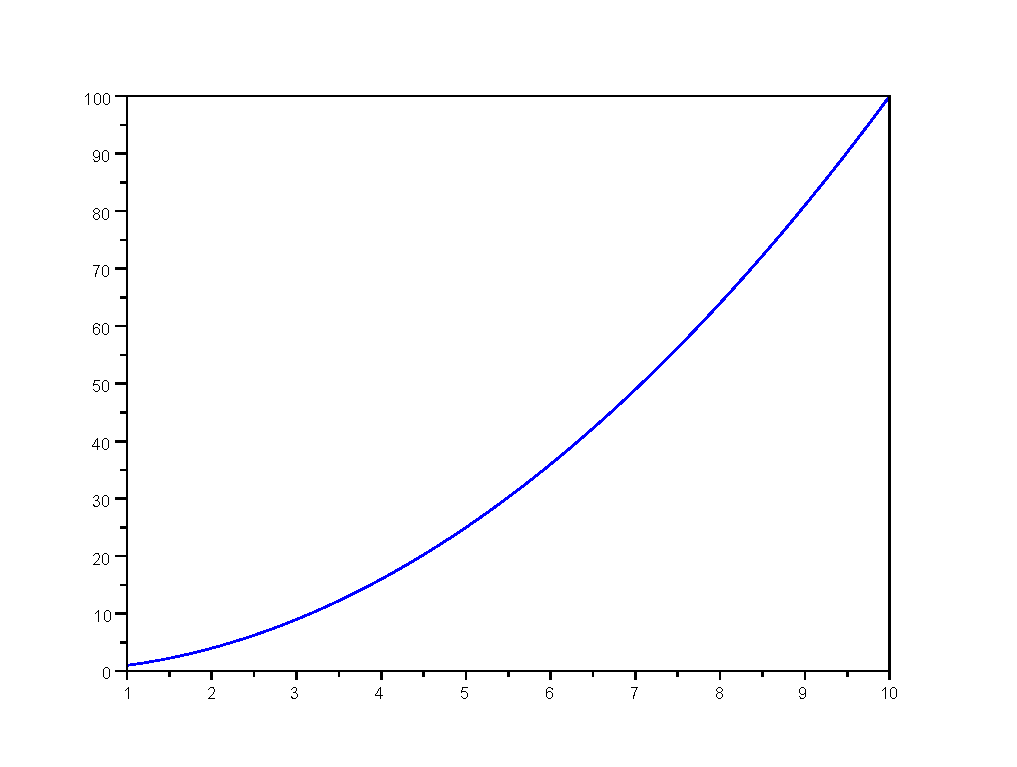
\includegraphics[width=10cm]{introscilab/xyplot.pdf}
\end{center}
\caption{A simple x-y plot.}
\label{fig-introoptim-xyplot}
\end{figure}

Notice that we could have produced the same plot without 
generating the intermediate array \scivar{ydata}.
Indeed, the second input argument of the \scifun{plot} function can
be a function, as in the following session.
\lstset{language=scilabscript}
\begin{lstlisting}
plot ( xdata , myquadratic )
\end{lstlisting}
When the number of points to manage is large, the previous syntax may
allow to save significant amount of time and memory space.

%%%%%%%%%%%%%%%%%%%%%%%%%%%%%%%%%%%%%%%%%%%%%%%%%%%%%%%%%%%%%%%%%
\subsection{Titles, axis and legends}

In this section, we present the Scilab graphics features
which allow to configure the title, axis and legends of 
an x-y plot. 

In the following example, we define a quadratic function and plot 
it with the \scifun{plot} function.
\lstset{language=scilabscript}
\begin{lstlisting}
function f = myquadratic ( x )
  f = x.^2
endfunction
xdata = linspace ( 1 , 10 , 50 );
ydata = myquadratic ( xdata );
plot ( xdata , ydata )
\end{lstlisting}

We have now the plot which is presented in figure \ref{fig-introoptim-xyplot}.

Scilab graphics system is based on \emph{graphics handles}.
The graphics handles provide an object-oriented access to the 
fields of a graphics entity. The graphics layout is decomposed into 
sub-objects such as the line associated with the curve, the x and y axis, 
the title, the legends, and so forth. Each object can be in turn decomposed 
into other objects if required. Each graphics object is associated 
with a collection of properties, such as the width or color of the line of the 
curve, for example. These properties can be queried 
and configured simply by setting or getting its value, as any other
Scilab variable. Managing handles is easy and very efficient.

But most basic plot configurations can be done by 
simple function calls and, in this section, we will focus in these 
basic features.

\index{\scifun{title}}
In the following script, we use the \scifun{title} 
function in order to configure the title of our plot.
\lstset{language=scilabscript}
\begin{lstlisting}
title ( "My title" );
\end{lstlisting}

\index{\scifun{xtitle}}
We may want to configure the axis of our plot as well.
For this purpose, we use the \scifun{xtitle} function 
in the following script.
\lstset{language=scilabscript}
\begin{lstlisting}
xtitle ( "My title" , "X axis" , "Y axis" );
\end{lstlisting}

The figure \ref{fig-introscilab-demotitle} presents the produced 
plot.

\begin{figure}
\begin{center}
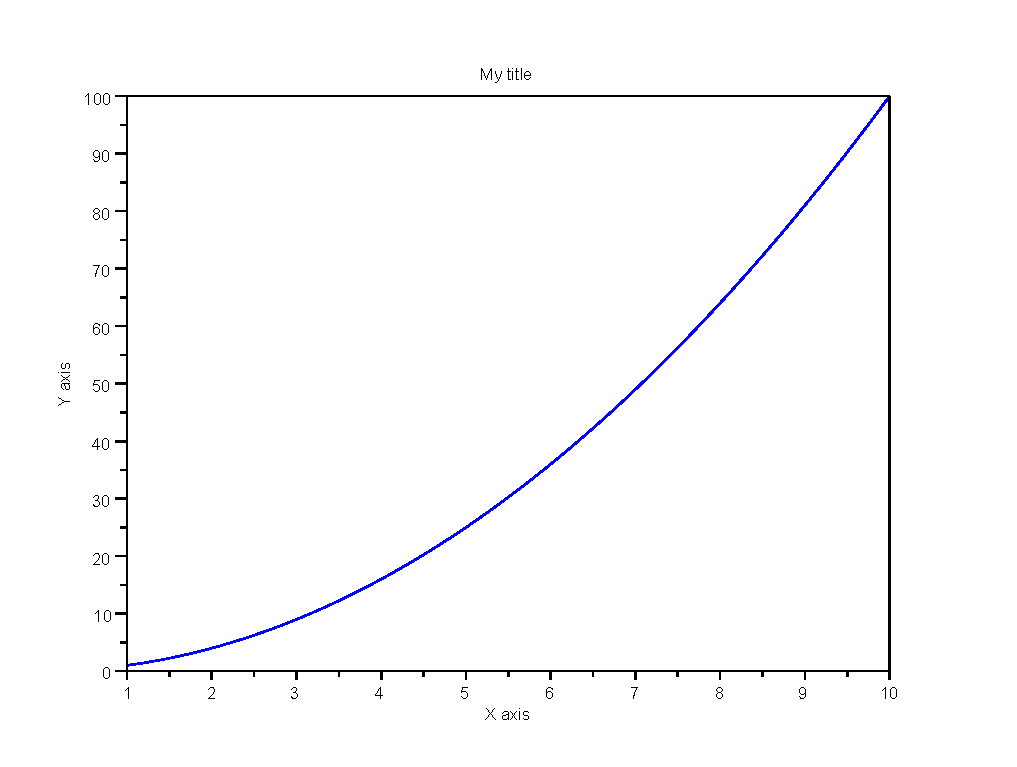
\includegraphics[width=10cm]{introscilab/xyplot_title.pdf}
\end{center}
\caption{The x-y plot of a quadratic function -- This is the same plot as in figure \ref{fig-introoptim-xyplot},
with title and x-y axis configured.}
\label{fig-introscilab-demotitle}
\end{figure}

It may happen that we want to compare two sets of datas in the 
same 2D plot, that is, one set of x data and two sets of y datas. 
In the following script, we define the two functions $f(x)=x^2$ and 
$f(x)=2x^2$ and plot the data on the same x-y plot.
We additionnaly add the "+-" and "o-" options to the \scifun{plot} function,
so that we can distinguish the two curves $f(x)=x^2$ and 
$f(x)=2x^2$.
\lstset{language=scilabscript}
\begin{lstlisting}
function f = myquadratic ( x )
  f = x^2
endfunction
function f = myquadratic2 ( x )
  f = 2 * x^2
endfunction
xdata = linspace ( 1 , 10 , 50 );
ydata = myquadratic ( xdata );
plot ( xdata , ydata , "+-" )
ydata2 = myquadratic2 ( xdata );
plot ( xdata , ydata2 , "o-" )
xtitle ( "My title" , "X axis" , "Y axis" );
\end{lstlisting}

%In order to configure the title and the x-y axis, we can 
%use the same commands as in the previous example.
Moreover, we must configure a legend so that we can know what curve 
is associated with $f(x)=x^2$ and what curve is associated with $f(x)=2x^2$.
For this purpose, we use the \scifun{legend} function in order to 
print the legend associated with each curve. 
%Notice that we pass the legends in the \emph{reverse} order of their creation:
%we pass first the legend "2x$\hat{\;}$2" for the $f(x)=2x^2$ plot (which has 
%been created last), and then the "x$\hat{\;}$2" legend for the $f(x)=x^2$ 
%(which has been created first).
\lstset{language=scilabscript}
\begin{lstlisting}
legend ( "x^2" , "2x^2" );
\end{lstlisting}

The figure \ref{fig-introscilab-demolegend} presents the produced x-y plot.
\begin{figure}
\begin{center}
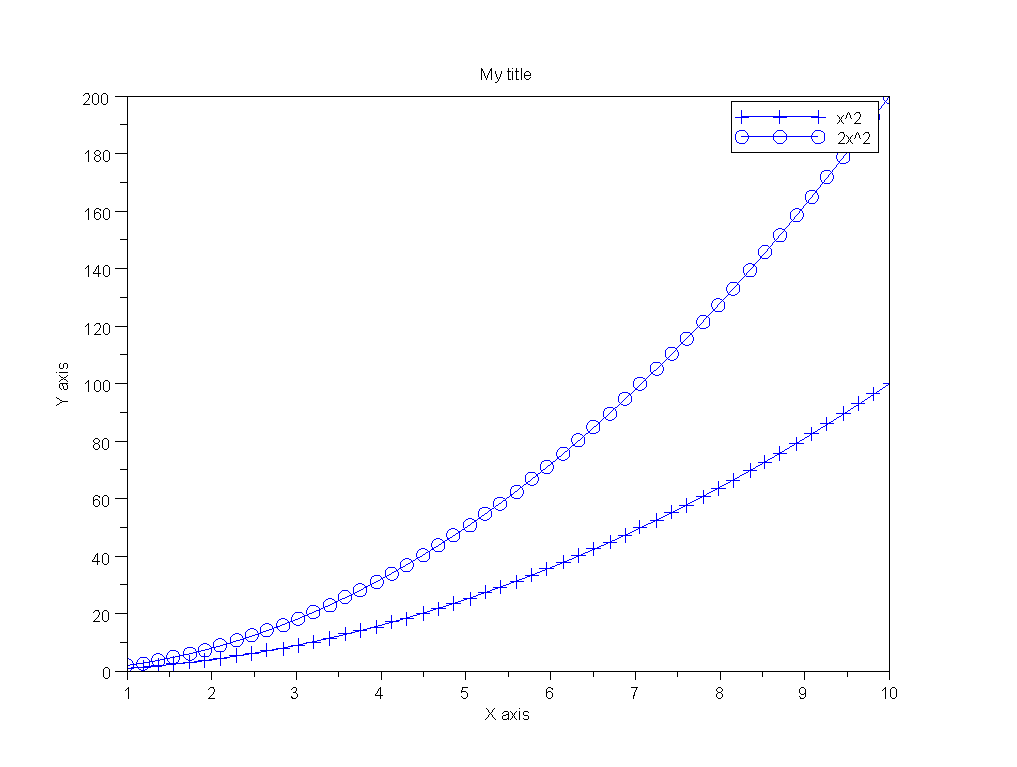
\includegraphics[width=10cm]{introscilab/xyplot_legend.pdf}
\end{center}
\caption{The x-y plot of two quadratic functions -- We have configured the legend so that 
we can distinguish the two functions $f(x)=x^2$ and $f(x)=2x^2$.}
\label{fig-introscilab-demolegend}
\end{figure}

We now know how to create a graphics plot and how to configure it.
If the plot is sufficiently interesting, it may be worth to put it into a report. 
To do so, we can export the plot 
into a file, which is the subject of the next section.

%%%%%%%%%%%%%%%%%%%%%%%%%%%%%%%%%%%%%%%%%%%%%%%%%%%%%%%%%%%%%%%%%
\subsection{Export}
In this section, we present ways of exporting 
plots into files, either interactively or 
automatically with Scilab functions.

Scilab can export any graphics into the 
vectorial and bitmap formats presented in figure \ref{fig-scilab-exportfile}.
Once a plot is produced, we can export its content into 
a file, by using interactively the \scimenu{File>Export to...} menu
of the graphics window. We can then set the name of the file and 
its type.


\begin{figure}
\begin{center}
\begin{tabular}{|l|l|}
\hline
\textbf{Vectorial} & \\
xs2png & export into PNG \\
xs2pdf & export into PDF \\
xs2svg & export into SVG \\
xs2eps & export into Encapsulated Postscript \\
xs2ps & export into Postscript \\
\hline
\textbf{Bitmap} & \\
xs2fig & export into FIG  \\
xs2gif & export into GIF  \\
xs2jpg & export into JPG  \\
xs2bmp & export into BMP  \\
xs2ppm & export into PPM \\
xs2emf & export into EMF  (only for Windows)\\
\hline
\end{tabular}
\end{center}
\caption{Export functions.}
\label{fig-scilab-exportfile}
\end{figure}

We can alternatively use the \scifun{xs2*} functions, presented in 
figure \ref{fig-scilab-exportfile}.
All these functions are based on the same following calling sequence:
\lstset{language=scilabscript}
\begin{lstlisting}
xs2png ( window_number , filename )
\end{lstlisting}
where \scivar{window\_number} is the number of the graphics window
and \scivar{filename} is the name of the file to export.
For example, the following session exports the plot which is in the 
graphics window number 0, which is the default graphics window,   
into the file \scifile{foo.png}.
\lstset{language=scilabscript}
\begin{lstlisting}
xs2png ( 0 , "foo.png" )
\end{lstlisting}

If we want to produce higher quality documents, the vectorial 
formats are to be prefered. For example, \LaTeX{} documents may use Scilab 
plots exported into PDF files to improve their readability, whatever
the size of the document.

%%%%%%%%%%%%%%%%%%%%%%%%%%%%%%%%%%%%%%%%%%%%%%%%%%%%%%%%%%%%%%%%%
\section{Notes and references}

There are a number of topics which have not been presented 
in this document. We hope that the current document is a good starting 
point for using Scilab so that learning about these specific 
topics should not be a problem. We have already mentioned a 
number of other sources of documentation for this purpose
at the begining of this document. 


Further reading may be obtained from the Scilab web cite \cite{WWWScilab},
in the documentation section.

\section{Acknowledgments}

I would like to thank Claude Gomez, Vincent Couvert, 
Allan Cornet and Serge Steer who let me share their comments about this document. 
I am also grateful to Julie Paul and Sylvestre Ledru who helped me during the writing 
of this document. 


%%%%%%%%%%%%%%%%%%%%%%%%%%%%%%%%%%%%%%%%%%%%%%%%%%%%%%%%%%%%%%%%%




%% Bibliography

\addcontentsline{toc}{section}{Bibliography}
\bibliographystyle{plain}
\bibliography{introscilab}

\addcontentsline{toc}{section}{Index}
\printindex

\end{document}

